\documentclass[12pt, a4paper]{book}%, oneside
\usepackage[printonlyused,withpage]{acronym}
\usepackage[headings]{fullpage}
\usepackage{setspace}

% \usepackage[top=1.5cm,right=1.5cm,bottom=1.5cm,left=1.5cm]{geometry}
% \usepackage{fancyhdr}
% \setlength{\headheight}{20pt} 
% \usepackage{graphics}
\usepackage{graphicx}
\usepackage{float}
\usepackage{subfig}
\usepackage{array}
\usepackage{arabtex}
\usepackage{utf8}
\setcode{utf8}
% \usepackage{xtab}
\usepackage{multirow}
\usepackage{booktabs}
\usepackage{appendix}
\usepackage[pdfborder={0 0 0}, colorlinks=true, linkcolor=black, citecolor=blue]{hyperref}
\usepackage[printonlyused]{acronym}
\usepackage{algorithmic}
\usepackage{algorithm}
\usepackage{ifpdf}
\usepackage{indentfirst}
\usepackage{listings}
\usepackage{minted}
\usepackage{color}
% \setlength{\parindent}{0pt}

\newcommand{\submissionDay}{XX}
\newcommand{\submissionMonth}{July}
\newcommand{\submissionYear}{20XX}
\newcommand{\submissionDate}{\submissionDay~\submissionMonth,~\submissionYear}
\newcommand{\typeOfThesis}{Bachelor Thesis}

\newcommand{\titleOfThesisOne}{Bachelor Thesis Title}

\newcommand{\authorOfThesis}{Author}
\newcommand{\supervisorOne}{Sup 1}
\newcommand{\supervisorTwo}{Sup 2}
\newcommand{\supervisorThree}{Sup 3}

\newcommand{\includefig}[4]{
    \begin{figure}[ht]
     \centering
      \includegraphics[width=#1\textwidth]{images/#2}
      \caption{#3}
      \label{#4}
    \end{figure}
}

\newcommand{\includefigWSC}[5]{
    \begin{figure}[ht]
     \centering
      \includegraphics[width=#1\textwidth]{images/#2}
      \caption[#3]{#4}
      \label{#5}
    \end{figure}
}

\newcommand{\includeeps}[4]{
\includefig{#1}{#2.eps}{#3}{#4}
}

\newcommand{\includeepsWSC}[5]{
\includefigWSC{#1}{#2.eps}{#3}{#4}{#5}
}


\ifpdf
\pdfinfo {
	/Author (\authorOfThesis)
	/Title (\titleOfThesisOne)
	/Subject (\typeOfThesis)
	/Keywords ()
	/CreationDate (D:20090707085533)
}
\fi
\definecolor{mygreen}{rgb}{0,0.6,0}
\definecolor{mygray}{rgb}{0.5,0.5,0.5}
\definecolor{mymauve}{rgb}{0.58,0,0.82}
\lstset{ %
  backgroundcolor=\color{white},   % choose the background color
  basicstyle=\footnotesize,        % size of fonts used for the code
  breaklines=true,                 % automatic line breaking only at whitespace
  captionpos=b,                    % sets the caption-position to bottom
  commentstyle=\color{mygreen},    % comment style
  escapeinside={\%*}{*)},          % if you want to add LaTeX within your code
  keywordstyle=\color{blue},       % keyword style
  stringstyle=\color{mymauve},     % string literal style
}
\begin{document}
% \overfullrule=5pt
\pagestyle{plain}
\pagenumbering{Roman}

\newcommand{\titlePage}{

\thispagestyle{empty}
\begin{center}
	\textbf{Media Engineering and Technology Faculty}\\[1mm]
	\textbf{German University in Cairo}\\[1mm]
	
\includegraphics[width=2.5cm]{GUC-logo-ss.eps}
	
	\vspace{2cm}
	\doublespacing
	{\Huge \textbf{Programming Language Localization}}\\
	\singlespacing
	\vspace{2cm}
	{\large \textbf{\typeOfThesis}}\\
	
	\vfill
	\parbox{1cm}{
  		\begin{large}
    			\begin{tabbing}
       			Author: \hspace{2cm}  
        			\= Omar Sherif El-Meteny\\[2mm]
      			Supervisors: 
        			\>Dr. Wael Abouelsaadat\\[2mm]
				
      			Submission Date: 
        			\>01 June, 2023\\
    			\end{tabbing}
  		\end{large}
	}\\
\end{center}
\clearpage
}
%++++++++++++++++++++++++++++++++++++++++++++++++++++++++++++++++++++
\titlePage
\thispagestyle{empty}\ \clearpage
\titlePage
%++++++++++++++++++++++++++++++++++++++++++++++++++++++++++++++++++++
\thispagestyle{empty}
This is to certify that:
\begin{itemize}
\item[(i)] the thesis comprises only my original work toward the Bachelor's Degree
\item[(ii)] due acknowledgments have been made in the text to all other material used
\end{itemize}

\vspace{2cm}
\begin{flushright}
\rule[0mm]{6cm}{0.2mm}\\
Omar Sherif El-Meteny\\
01 June, 2023\\
\end{flushright}
\clearpage


\chapter*{Acknowledgments}
\addcontentsline{toc}{chapter}{Acknowledgments}
\label{chap:ack}
This project wouldn't have been done without the assistance and support of many people. First and foremost, thanks to God almighty for everything I have and know. Next, I would like to thank Dr. Wael Abouelsaadat for guiding me throughout the semester and giving me constructive feedback that helped in improving the project. I would like to thank all my teachers and instructors at school and university who generously shared their knowledge with me. Finally, I would like to thank my parents, brother, and friends for always supporting me whenever I needed them which gave me more motivation and confidence.


\chapter*{Abstract}
% \addcontentsline{toc}{chapter}{Abstract}
\label{chap:abstract}
Abstact

\tableofcontents
% \addcontentsline{toc}{chapter}{Contents}
\clearpage 

\pagestyle{headings}
\pagenumbering{arabic}

% \setlength\parskip{15pt}
\setlength\parskip{.5\baselineskip plus .2\baselineskip
	minus .4\baselineskip}
% \setlength\parskip{.5\baselineskip \@plus .1\baselineskip \@minus ..1\baselineskip}

\chapter{Introduction}
\section{Motivation}
Computer programming is of the most significant importance in today's digital age because it plays a significant role in various aspects of our lives and has a remarkable impact on numerous industries and fields. It is essential due to its problem-solving capabilities, automation potential, fostering innovation, offering career opportunities, enhancing digital literacy, promoting computational thinking, enabling interdisciplinary applications, and empowering individuals. As technology advances, programming skills will become increasingly valuable in shaping the future. 

In the Islamic golden age, Arabic played a significant role as the language of sciences. Arab scholars and scientists made significant contributions in various fields, such as mathematics, astronomy, medicine, chemistry, physics, and philosophy. The wide spread of Arabic has faded away, and currently, English is the most prominent language, especially in the field of computer science. This created a barrier for non-English speakers to delve into the field of computer programming. My aim is to remove this barrier.
\section{Problem Statement}
Nowadays, almost all programming languages are in English, so a person must learn English before learning computer programming. This project aims to eliminate the need to learn English because anyone can write programs using their native language. This will be done by localizing the Java Programming Language.
\section{Thesis Organization}
This paper consists of four chapters. Chapter One is the Introduction, chapter two is the Literature Review and is divided into two sections: Background and Previous Work for Programming Language Localization, chapter three covers the Design and Implementation of the system and is divided into five sections: Project Goals, Project Overview, Design Approach, Implementation Details, and Deploying and Packaging the Eclipse Plugin, and finally chapter four is the Conclusion, and it is divided into three sections: Achievements, Limitations of the project, and Future Work which are features that can be added to the project.


% add more chapters here


\chapter{Literature Review}\label{chap:Literature Review}
\section{Background}
Throughout the history of computer programming, most programming languages have been based on the English Language. However, the first-ever high-level programming language, "Plankalkül," designed by German Civil Engineer Konrad Zuse, was based on the German language \cite{arawjo2020write}. This programming language was designed mainly to replace Assembly language because it was noticed that it requires a great amount of mental effort. One of the advantages of high-level programming languages was that short code statements represented mathematical expressions in an understandable and readable form. Finally, the program written using high-level programming language had to be interpreted to machine code every time it ran, making the process match slower than running the equivalent machine code directly.

Different approaches to programming have evolved gradually. The programming paradigm concept began to rise. The first paradigm was the lowest-level programming paradigm, which was machine code that represented instructions in binary format. The next paradigm developed was the procedural paradigm. These languages (high-level languages) use vocabulary related to the problem being solved, and they describe exactly the procedure that should be followed to solve a specific problem. Then the \ac{OOP} languages were created, and in these languages, data and methods to manipulate it are kept as one entity called an object. In OOP, the only way to access the data is through the object's methods, guaranteeing flawless encapsulation. Then there were further programming paradigms, including imperative programming, declarative programming, functional programming, logic programming, and symbolic programming. Imperative programming is structured as a human-centered web, while declarative programming languages tell the computer what the problem is instead of telling how to solve it. Functional programming uses functions and recursion rather than assigning variables, while logic programming views computation as automated reasoning. Symbolic programming allows programs to manipulate formulas and program components as data. Finally, differentiable programming structures programs so they can be differentiated throughout \cite{programmingparadigms}.

Many attempts were made to design and implement localized programming languages. In order to design a localized language or understand how it is designed, I must first understand the tools and components needed to build a programming language.

A scanner (or lexer) takes the source code as a stream of characters and assembles them into individual tokens. These tokens can be single characters like ( and, or multi-character sequences like numbers (123), string literals ("hi!"), and identifiers (min).
Certain characters in a source file are not important. Whitespace is usually irrelevant (with Python being one of the notable exceptions), and comments are disregarded by the language by definition. The scanner typically discards these, leaving only meaningful tokens in a clean sequence \cite{nystrom2021crafting}. For example:
\begin{figure}[ht]
\centering

\includegraphics[width=15cm]{ch2-images/source-ccode.png}
\caption{Source Code \cite{nystrom2021crafting}}
\label{fig:Source Code}
\end{figure}

A lexer would turn the above code into the following set of tokens:
\begin{figure}[ht]
\centering

\includegraphics[width=15cm]{ch2-images/tokens.png}
\caption{Tokens \cite{nystrom2021crafting}}
\label{fig:Tokens}
\end{figure}

After scanning the source code, the next step for code processing is parsing. A parser takes the tokens generated by the lexer and constructs a parse tree (also called \ac{AST}) which reflects the language's grammar. For example, the above set of tokens is turned into the following tree:
\begin{figure}[ht]
\centering
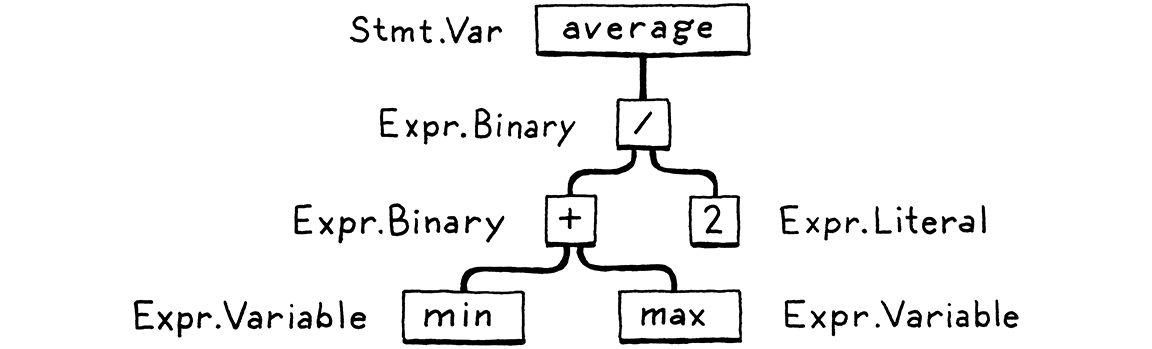
\includegraphics[width=15cm]{ch2-images/parser.png}
\caption{Syntax Tree \cite{nystrom2021crafting}}
\label{fig:Syntax Tree}
\end{figure}

It’s also the parser's job to detect code that violates the grammar rules of the language and report syntax errors.
Some language implementations have a tree-walk interpreter that traverses the AST to run the program. Other language implementations can use the syntax tree to transpile the program to a different high-level programming language \cite{nystrom2021crafting}.

After parsing the AST, the next step for code processing is the static analysis. A static analyzer uses the AST to perform binding and scope resolution, which determines what an identifier refers to. If the language is statically typed, type checking occurs at this stage, and type errors are reported if the language rules are violated.

The lexer, parser, and static analyzer are called the front end of the language implementation.

The last two steps are code optimization and code generation. Code optimization is replacing a line of code or a group of lines with a different code which is more efficient than the code written by the user as it uses less memory and runs faster. This step takes place just before generating the code. Finally, code generation takes place where a compiler generates the program's equivalent bytecode, which is then converted to machine code for a target processor architecture and operating system, or a transpiler which generates code in a target high-level programming language \cite{nystrom2021crafting}.

The code optimizer and the code generator are called the back end of the language implementation.

The following figure includes all parts of a programming language and summarizes the process of building a new programming language:
\begin{figure}[ht]
\centering
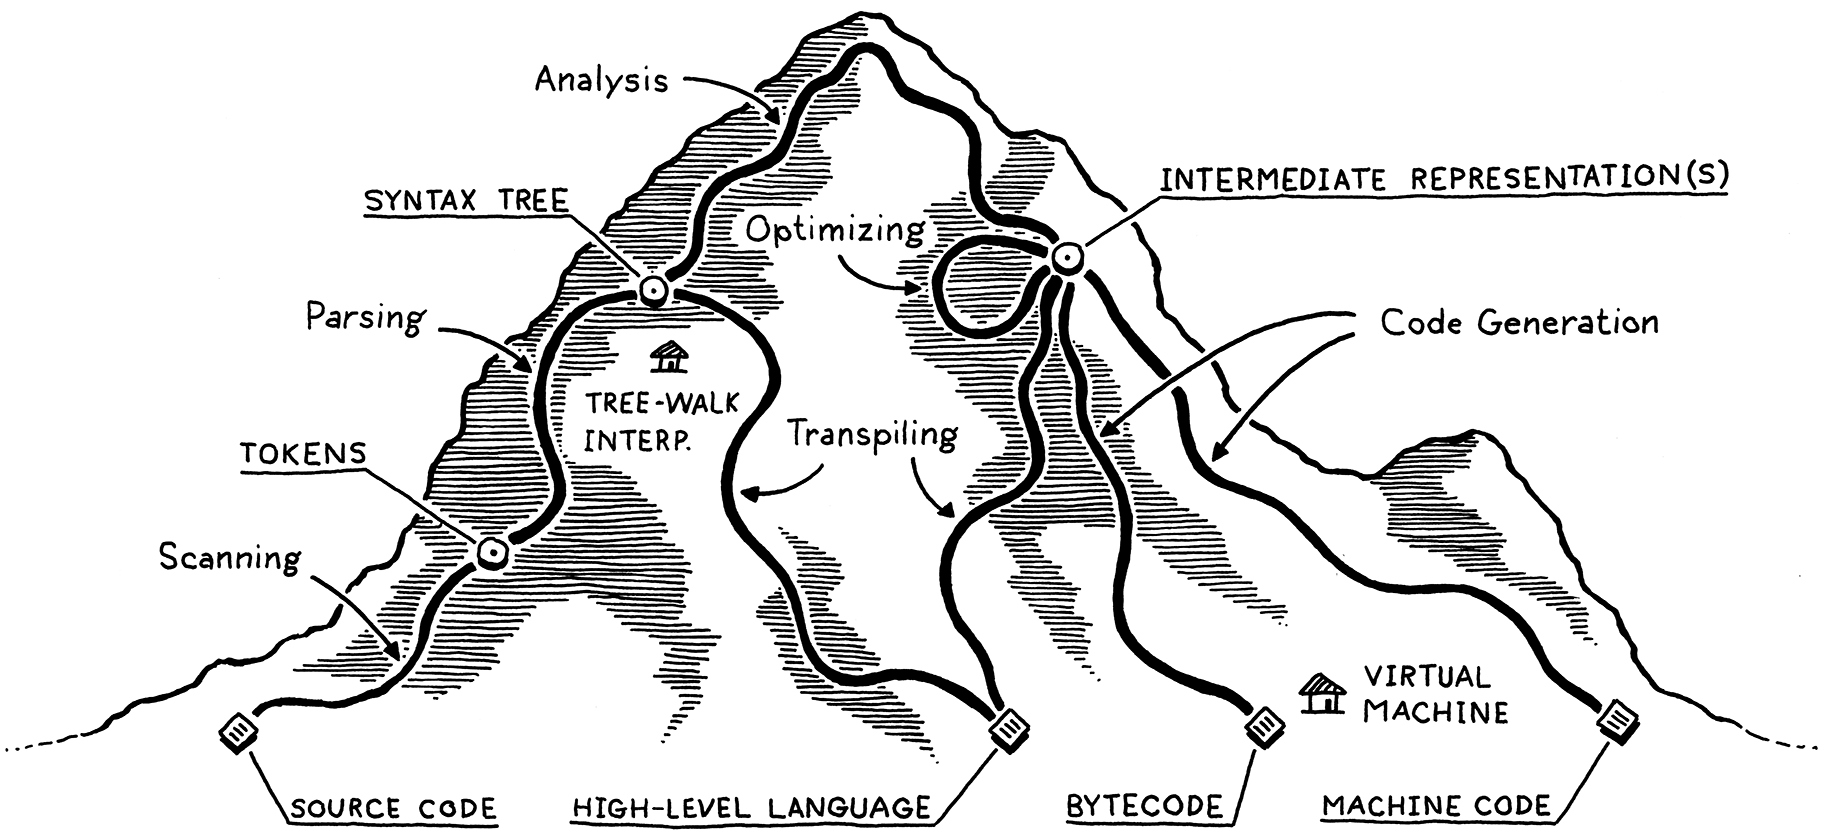
\includegraphics[width=15cm]{ch2-images/mountain.png}
\caption{Programming Language Mountain \cite{nystrom2021crafting}}
\label{fig:Programming Language Mountain}
\end{figure}

In order to use a programming language in writing a program, a code editor must be used. A code editor is an application used to edit source code. It typically includes features like syntax highlighting, code completion, and a debugger. An \ac{IDE} is an application that includes a code editor and other features like tools for unit testing, issue tracking, etc.

Eclipse is one of the most well-known IDEs for computer programming, with a base workspace and a customizable plugin system. Eclipse is mainly used for Java development but can also be used for other programming languages through plugins, such as C++, Python, PHP, and other languages. Eclipse is written mostly in Java, and its \ac{SDK}, which is a set of tools to build software for a particular platform, is free and open-source software released under the Eclipse Public License. Moreover, it allows users to write and contribute their own plugin modules \cite{eclipseide}.

Eclipse Plugins are computer programs that can be included with Eclipse to increase functionality and personalize the workspace. New features and functionalities, including support for additional programming languages, testing frameworks, and build systems, as well as new user interfaces and visualizations, can be offered via these plugins. Plugins can be downloaded and manually installed, or they can be installed and managed using the Eclipse Marketplace. Eclipse's extensible plugin design enables programmers to create and share their own plugins with the community \cite{eclipseplugins}.
\section{Previous Work for Programming Language Localization}
As mentioned before, many attempts were made to design a localized programming language in Arabic and other languages. In this section, I will discuss some of the previous work to localize a programming language or implement a non-English programming language.
\subsection{Babylscript}
 Iu \cite{iu2011babylscript} created Babylscript, which is a multilingual version of JavaScript. It allows programmers to write code using several languages and transition between language modes while doing so. By allowing several names to be attached to a single data item, Babylscript improves characteristics and makes it possible to create libraries with translated functions and object names for different languages. The following figure shows an example of Babylscript code:
\begin{figure}[ht]
\centering
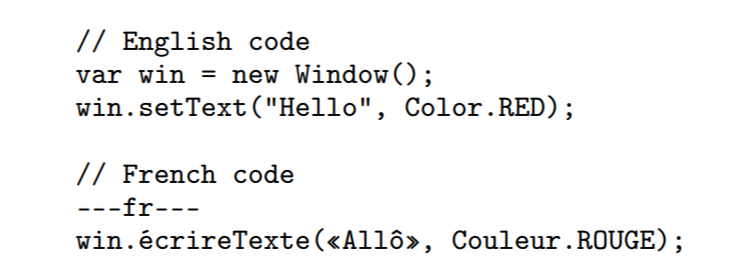
\includegraphics[width=10cm]{ch2-images/babylscript.png}
\caption{Babylscript Code \cite{iu2011babylscript}}
\label{fig:Babylscript Code}
\end{figure}

The architecture of Babylscript is based on the observation that punctuation and mathematical notations are shared by all natural languages. Therefore, it has a syntax that all languages share. Babylscript shares the same grammar for all language modes, despite the fact that various language modes may use different names for functions, objects, and methods as well as distinct tokens for keywords and operations. To switch between different language modes, programmers must write a command using three minus signs followed by the language they want to use followed by another three minus signs (see figure \ref{fig:Babylscript Code}). All keywords and symbols are translated into the new language as soon as the programmer switches the language mode. By enabling properties to have more than one translation in addition to their default name, Babylscript enhances the JavaScript object model. Therefore, if a translated name is available, programmers can access any property using that name instead of the default one. The following figure shows an example of property translation:

\begin{figure}[H]
\centering
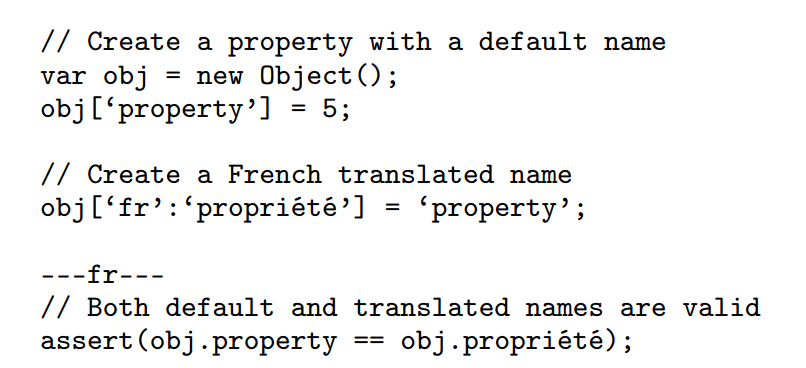
\includegraphics{ch2-images/babylscript2.png}
\caption{Babylscript Property Translation \cite{iu2011babylscript}}
\label{fig:Babylscript Property Translation}
\end{figure}

Babylscript is an extension of Mozilla Rhino JavaScript interpreter that uses the same parser, bytecode generator, and bytecode for all language modes because it uses the same grammar for all languages. However, each language has its own tokenizer to identify keywords and other tokens. Language context must be tracked by Babylscript's compiler because the access of properties of an object is dependent on the language mode. This is done by adding language tags to all structures passed between stages of the compiler. During tokenization, Babylscript's tokenizers convert keywords into a standard form, such as English, while leaving identifiers untouched. Since JavaScript names are resolved at runtime, the interpreter requires the language tags to detect the correct table of translated names for an object. The following figure shows how Babylscript is designed:
\begin{figure}[H]
\centering
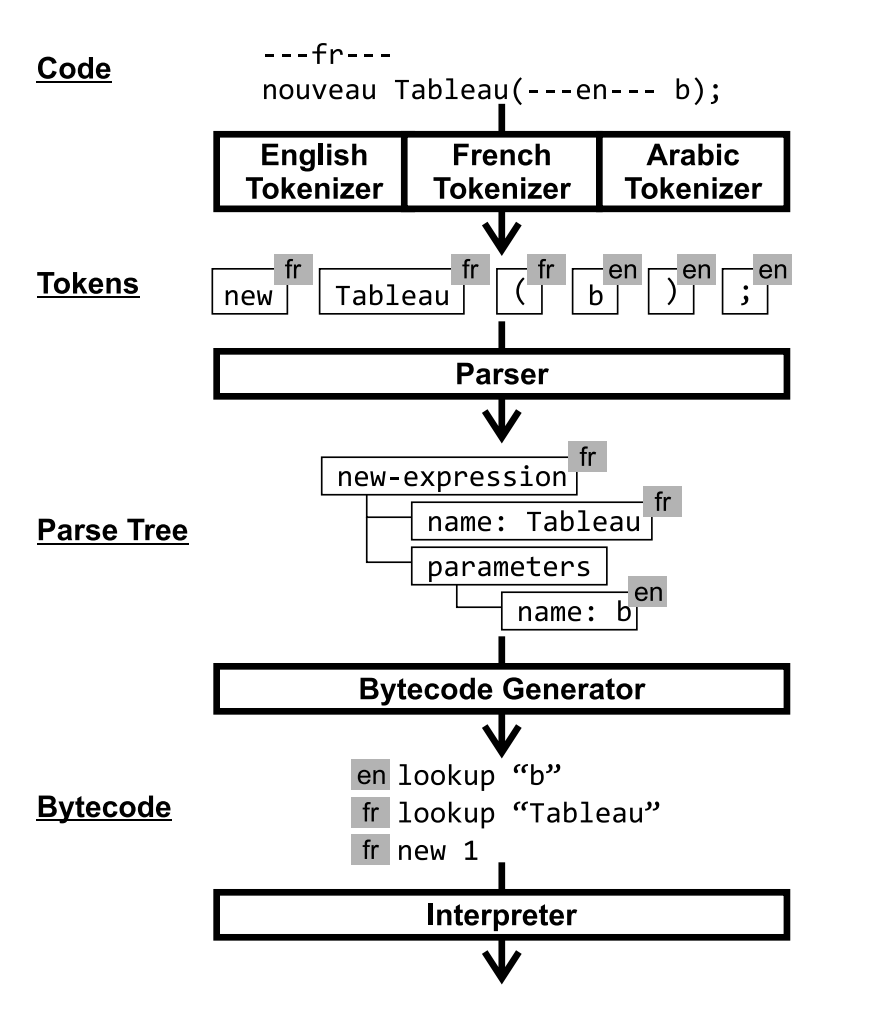
\includegraphics[width=7.3cm]{ch2-images/babylscript3.png}
\caption{Babylscript Implementation \cite{iu2011babylscript}}
\label{fig:Babylscript Implementation}
\end{figure}

Babylscript's language design allows programmers to write code using their own native language without being aware of Babylscript's support for other languages. In the future, some of the ideas behind Babylscript could be applied to statically typed languages like Java.
\subsection{Phoenix}
 Bassil \cite{bassil2019phoenix} created Phoenix, which is a computer programming language based on Arabic. It is a compiled, object-oriented, high-level, imperative, and general-purpose programming language. Phoenix is regarded as a C\# programming language localization. Both share the same syntax, and Phoenix uses features of modern languages to make Arabic programming easier. Phoenix is compiled from source code to machine code before being executed, just like C\#. Its current version runs on the Windows operating system and has the ability to convert compiled machine code into an executable file. Phoenix also comes with a suitable and user-friendly IDE that enables developers to write, save, debug, and compile their source code.

Phoenix is a modern programming language that offers many features that are suitable for computer programming. It includes supporting strong data types such as Decimal, String, Recursion, implicit type conversion between data types, conditional structures (if and if-else), and many other features.

The Phoenix compiler consists of six building blocks: preprocessor, scanner, parser, semantic analyzer, code generator, and linker. Each of these blocks will be discussed in detail.

The preprocessor helps in code simplification by eliminating extra information from the source code, including code comments and unneeded variables, and integrating third-party libraries. The scanner then tokenizes the simplified source code into understandable units known as tokens. The parser then examines the tokens created by the scanner to see if they comply with the programming language's syntax and grammar. The Phoenix parser is based on a \ac{CFG} as it provides powerful features including but not limited to recursion and nesting. The semantic analyzer then checks whether the code follows the semantics of the language, and then the parse tree is translated into executable code by the code generator. This code could be bytecode, machine code, or any other high-level programming language. Finally, the linker converts the target code into a stand-alone executable that can run on the operating system. 

The algorithm of the scanner is based on the \ac{FSM} to detect and tokenize identifier/variable names, numeric values, and string values, respectively. Phoenix keywords are also detected by the scanner. The following figures show the FSMs mentioned:

\begin{figure}[H]
\centering
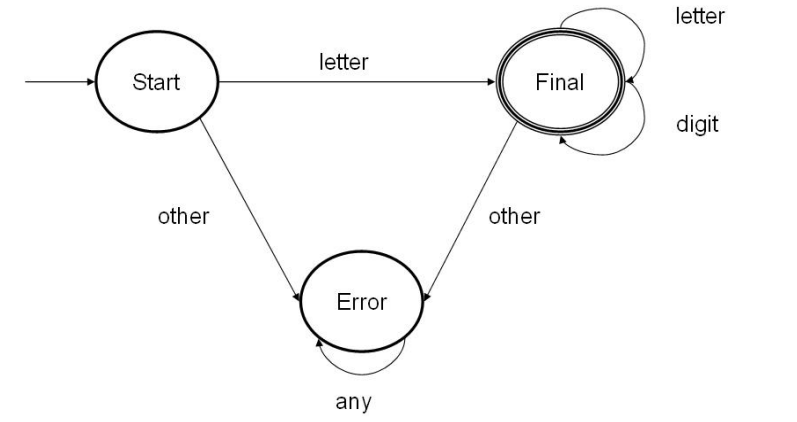
\includegraphics[width=10cm]{ch2-images/phoenix.png}
\caption{Finite Automata for Identifiers \cite{bassil2019phoenix}}
\label{fig:Finite Automata for Identifiers}
\end{figure}

\begin{figure}[H]
\centering
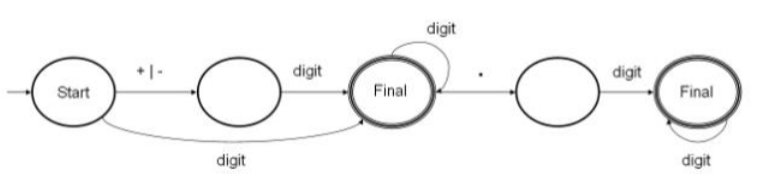
\includegraphics[width=10cm]{ch2-images/phoenix2.png}
\caption{Finite Automata for Numeric Values \cite{bassil2019phoenix}}
\label{fig:Finite Automata for Numeric Values}
\end{figure}

\begin{figure}[H]
\centering
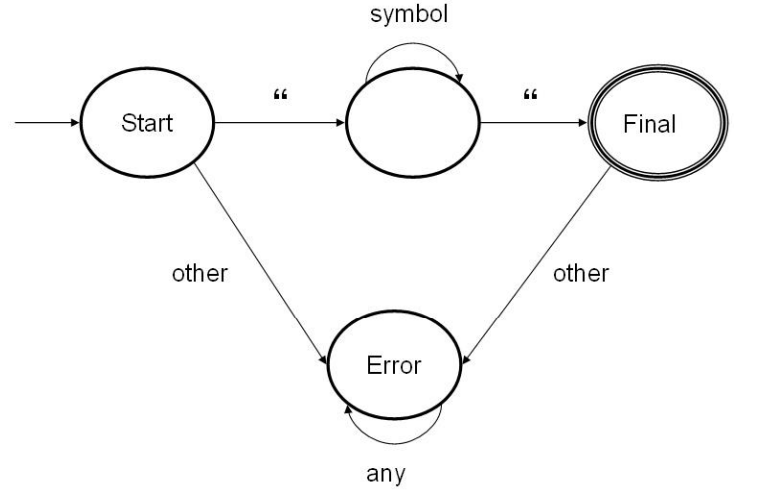
\includegraphics[width=10cm]{ch2-images/phoenix3.png}
\caption{Finite Automata for String Values \cite{bassil2019phoenix}}
\label{fig:Finite Automata for String Values}
\end{figure}

In the following figures, we will see a sample code written using Phoenix in an IDE designed especially for Phoenix and its equivalent C\# code:

\begin{figure}[H]
\centering
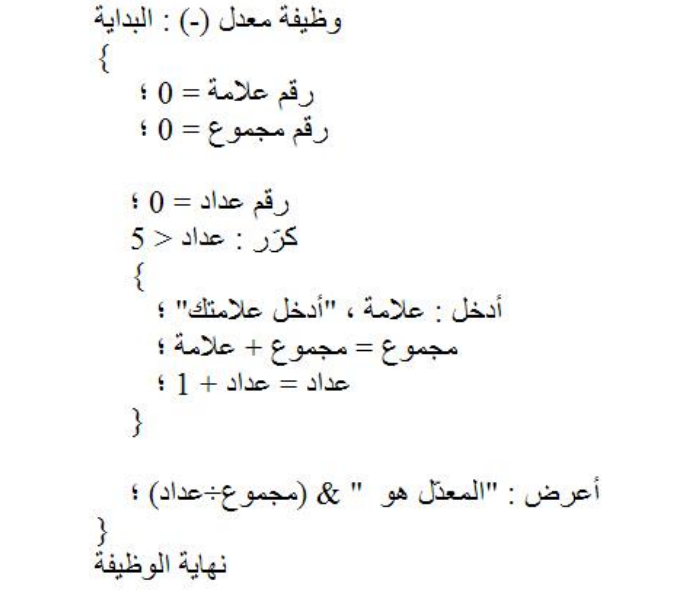
\includegraphics[width=8.5cm]{ch2-images/phoenix4.png}
\caption{Source code written using Phoenix \cite{bassil2019phoenix}}
\label{fig:Source code written using Phoenix}
\end{figure}

\begin{figure}[H]
\centering
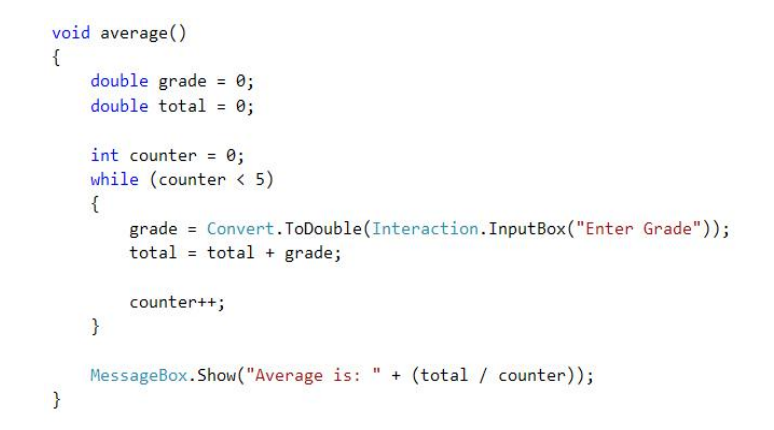
\includegraphics[width=15cm]{ch2-images/phoenix5.png}
\caption{Equivalent Source-Code written using C\# \cite{bassil2019phoenix}}
\label{fig:Equivalent Source-Code written using C\#}
\end{figure}

The results have shown several powerful features of Phoenix, including functions, while-loop, and arithmetic operations and its capability to build general-purpose programs that can be used for real-world applications. Phoenix might eventually get some additional object-oriented features, including inheritance, encapsulation, abstraction, and polymorphism. Additionally, a library of built-in classes and reusable functions is to be created with the aim of supplying several functionalities like file processing and database access.
\subsection{ARABLAN}
Al-A’ali and Hamid \cite{al1996design} created ARABLAN (or ARABLANG) which is another example of an Arabic programming language. It is a localization of Pascal programming language, and its mainly designed for non-English speaking school students to develop their computer programming skills. Learning ARABLAN is challenging for those whose native language is neither English nor Arabic. 

A few design decisions must be made while creating a programming language. In fact, various design decisions were made for ARABLAN, such as making it a high-level, sequential, imperative, and simple language to learn. The language uses relevant Arabic words that are simple to recall to make it simple to learn. Additionally, it achieves mobility and portability via the popular and affordable Arabic interface tool ``Nafitha." 

The syntax of the ARABLAN language is built with efficiency for both translation and execution. This is accomplished by adhering to certain rules, such as avoiding backtracking during parsing, ensuring an unambiguous grammar, avoiding dynamic storage allocation, using an appropriate internal form that can be executed directly, and reserving specific words for designated usages. 

The language allows the creation of two distinct types of declarations: constant declarations and variable declarations. An ARABLAN program begins with the declarations section, which is followed by the main program section, which contains the statements that can be executed. There are different types of statements, including assignment statements, selection statements, repetition statements, and input/output statements. Moreover, programmers can write subprograms in ARABLAN, which are parts of the main program. There are two different types of subprograms just like Pascal. 

The first two figures are two examples explaining the two types of declaration. The first figure is an example of the Constants Declaration, while the second figure is an example of the Variables Declaration:

\begin{figure}[h]
\centering
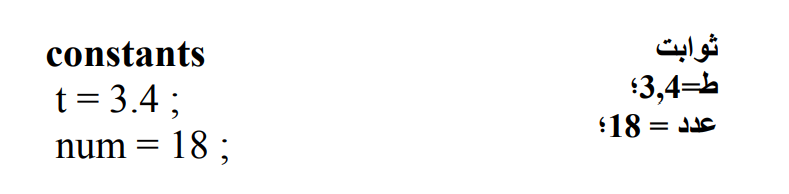
\includegraphics[width=8cm]{ch2-images/ARABLAN.png}
\caption{ARABLAN Constants Declaration \cite{al2007evaluation}}
\label{fig:ARABLAN Constants Declaration}
\end{figure}

\begin{figure}[h]
\centering

\includegraphics[width=8cm]{ch2-images/ARABLAN2.png}
\caption{ARABLAN Variables Declaration \cite{al2007evaluation}}
\label{fig:ARABLAN Variables Declaration}
\end{figure}

The following six figures represent the structure of a program written in ARABLAN and examples of the different kinds of statements that could be written in the program:

\begin{figure}[H]
\centering

\includegraphics[width=10cm]{ch2-images/ARABLAN3.png}
\caption{ARABLAN Program \cite{al2007evaluation}}
\label{fig:ARABLAN Program}
\end{figure}

\begin{figure}[H]
\centering

\includegraphics[width=10cm]{ch2-images/ARABLAN4.png}
\caption{ARABLAN Assignment Statement \cite{al2007evaluation}}
\label{fig:ARABLAN Assignment Statement}
\end{figure}

\begin{figure}[H]
\centering
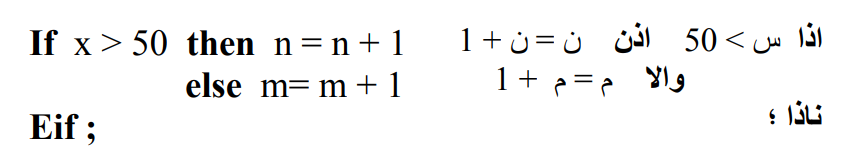
\includegraphics[width=10cm]{ch2-images/ARABLAN5.png}
\caption{ARABLAN Selection Statement \cite{al2007evaluation}}
\label{fig:ARABLAN Selection Statement}
\end{figure}

\begin{figure}[H]
\centering
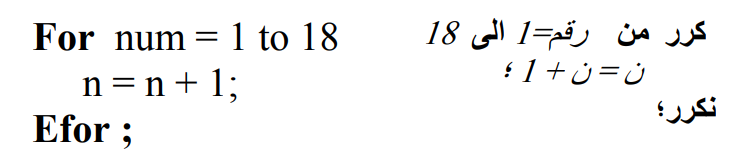
\includegraphics[width=10cm]{ch2-images/ARABLAN6.png}
\caption{ARABLAN Repetition Statement (For loop) \cite{al2007evaluation}}
\label{fig:ARABLAN Repetition Statement (For loop)}
\end{figure}

\begin{figure}[H]
\centering
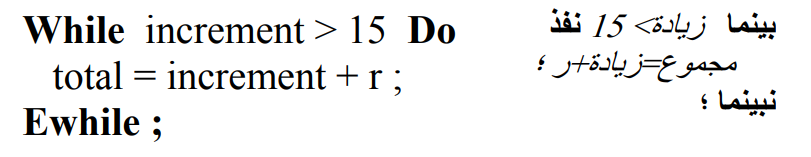
\includegraphics[width=10cm]{ch2-images/ARABLAN7.png}
\caption{ARABLAN Repetition Statement (While loop) \cite{al2007evaluation}}
\label{fig:ARABLAN Repetition Statement (while loop)}
\end{figure}

\begin{figure}[H]
\centering

\includegraphics[width=10cm]{ch2-images/ARABLAN8.png}
\caption{ARABLAN Input/Output Statement \cite{al2007evaluation}}
\label{fig:ARABLAN Input/Output Statement}
\end{figure}

Finally, the last figure represents an example illustrating the structure of a subprogram in ARABLAN:

\begin{figure}[H]
\centering
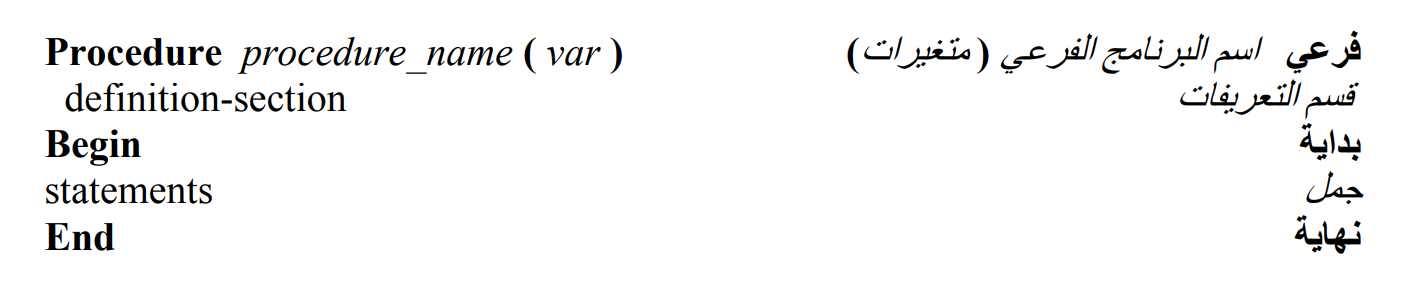
\includegraphics[width=15cm]{ch2-images/ARABLAN9.png}
\caption{ARABLAN Subprograms \cite{al2007evaluation}}
\label{fig:ARABLAN Subprograms}
\end{figure}

ARABLAN was put to the test in Bahrain schools to find out how well it taught Arab children computer programming. These studies and assessments aimed to establish whether ARABLAN was simple or challenging for pupils to learn. Additionally, homework assignments and data on students' language use were given to the students, and several language keywords were modified as a result of the statistics. For instance, the majority of pupils preferred using \<الثوابت> rather than \<ثوابت>. Consequently, this keyword was one of those that was altered in the language's syntax. Surveys were conducted to find out whether students prefer programming in their own language or in another language. The results showed that the majority of students preferred using Arabic. 

Results demonstrated that ARABLAN is clearly a step in the right direction for the future of Arabic programming languages. Numerous other elements of Arabic programming, such as the selection of terminology and mnemonics, the starting level, and so forth, need further study. Dr. Hamid tragically passed away suddenly just before finishing the study that he and Dr. Mansoor Al-A'ali had begun \cite{al2007evaluation}.
\subsection{DHAD}
Ben Othman \cite{othman2016arabic} created DHAD, which is another Arabic programming language. It aims to help non-English speaking students learn computer programming. DHAD is constructed in stages and has a number of parts. DHAD contains a compiler that converts source code into machine, C, and Assembly languages. A very useful editor is also available for writing programs using DHAD. Learning DHAD became an easy process because there is an interactive user interface that guides the user in learning DHAD through different complexity levels. The Exams component is one of the special components in DHAD’s architecture because it can be used by the instructor to create exams for their students. Here is a figure that shows the DHAD's architecture:
\begin{figure}[H]
\centering
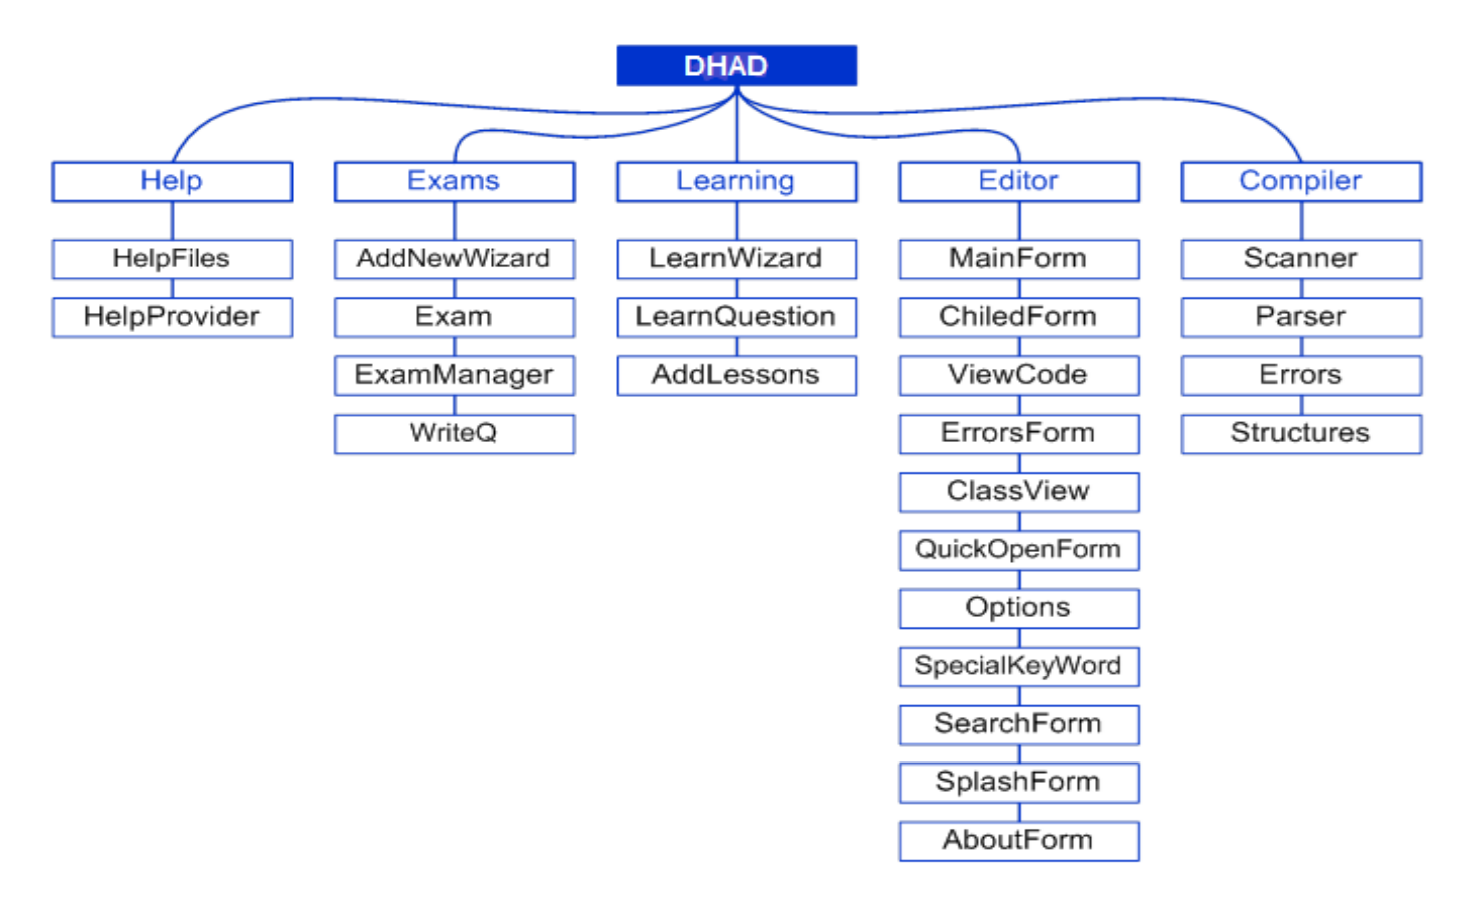
\includegraphics[width=8cm]{ch2-images/DHAD.png}
\caption{DHAD Tool’s Architecture \cite{othman2016arabic}}
\label{fig:DHAD Tool’s Architecture}
\end{figure}

A language's grammar must be decided before the compiler is created. The grammar is a combination of numerous high-level programming languages, including C, C++, and Pascal. It is the responsibility of the compiler to accept a file with the ".apl" extension (which stands for Arabic Programming Language) as input and construct the output files ``filename.c" and ``filename.asm" which contain translations of the written programs into C and Assembly, respectively. Depending on the compiler choices, different results are produced. The following figure explains the compiler's structure:

\begin{figure}[H]
\centering
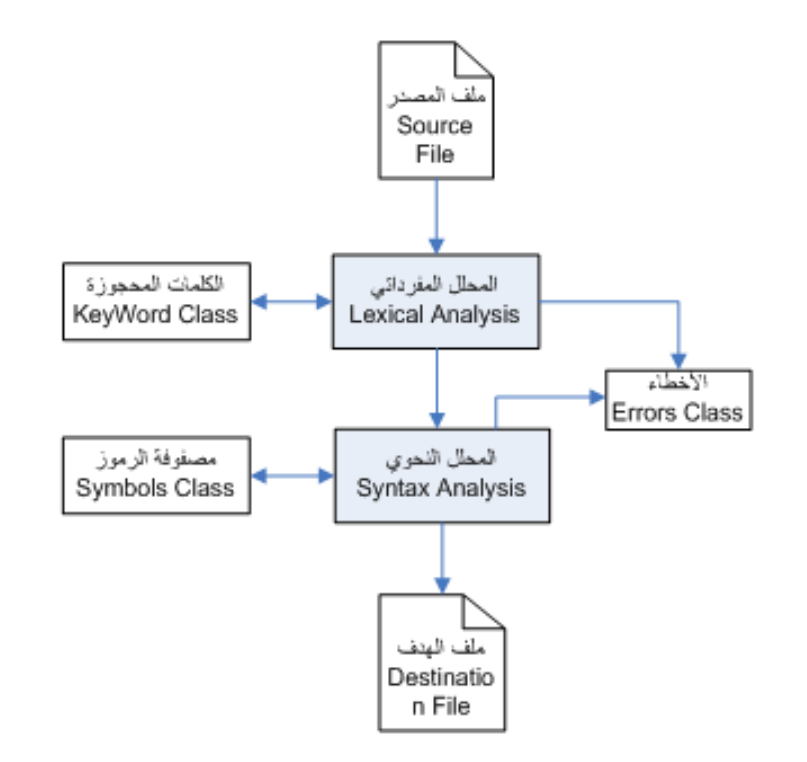
\includegraphics[width=8cm]{ch2-images/DHAD2.png}
\caption{DHAD Compiler's Structure \cite{othman2016arabic}}
\label{fig:DHAD Compiler's Structure}
\end{figure}

The syntax of DHAD is taken from three different languages which are C, C++, and Pascal, and modified to be easily used and understood by students later on. The following table gives some default keywords chosen for the DHAD programming language:

\begin{figure}[ht]
\centering
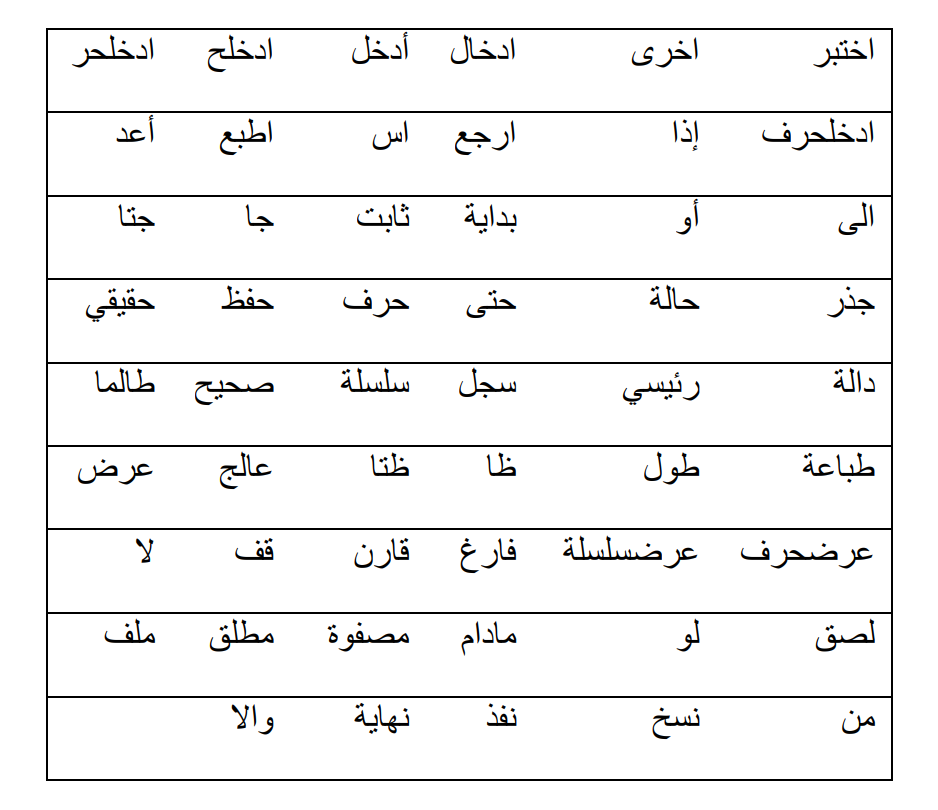
\includegraphics[width=10cm]{ch2-images/DHAD3.png}
\caption{DHAD Language Keywords \cite{othman2016arabic}}
\label{fig:DHAD Language Keywords}
\end{figure}

Multiple modules make up the compiler for DHAD. Prior to sending the tokens to the parser, the lexer must first read the program as a stream of characters and create tokens. The parser, which was developed according to the grammar of the language, determines whether the tokens sent by the lexer adhere to the grammar rules. The third module is then called by the parser, and if there are no syntax mistakes, it converts the source code to the target language.

The editor that supports the DHAD programming language has a help menu containing instructions' syntaxes with examples, a file menu for file management, and a compile menu with options for translation to C, Assembly language, and machine language. The program also allows users to customize keywords, giving them the ability to change any keyword in the language and revert back to the default keywords. 

Executing the program in the editor could be done in different ways. First, the direct execution in which the program is directly translated into machine language and then executed on the machine's processor. Another way is the cross-language translation in which the program is translated to Assembly or C according to the user's choice. DHAD has its own assembler that can be used separately, and then all messages like warnings, errors, and help are written in Arabic. Moreover, this assembler converts the translated Assembly code to machine language to be executed.

Future work on DHAD will concentrate mainly on how students could modify the code to have their own grammar rules for the compiler and their own control modules in the operating system.
\subsection{Alf..Eih}
Another Arabic programming language called Alf..Eih was created by Abdul Razaq et al \cite{razaq2019designing}. The decision to develop this language was contested. The usage of Arabic programming languages is impractical, according to opponents, who also said that any computer program should only be developed using English programming languages. On the other side, proponents asserted that there must be a programming language that fits the culture of the users. The following figure shows the general form of Alf..Eih:

\begin{figure}[H]
\centering
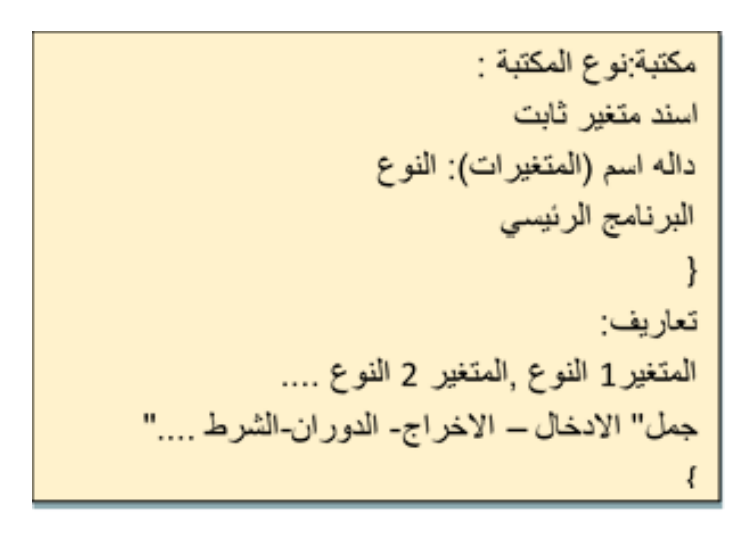
\includegraphics[width=10cm]{ch2-images/AlfEih.png}
\caption{Alf..Eih Program \cite{razaq2019designing}}
\label{fig:Alf..Eih Program}
\end{figure}

Alf..Eih is a localization of C++ programming language. This is done bearing in mind a non-expert user that can learn the language using simple ideas. The process of implementation involves a number of steps that will be discussed. The following figure shows an overview of the stages of implementation:

\begin{figure}[H]
\centering
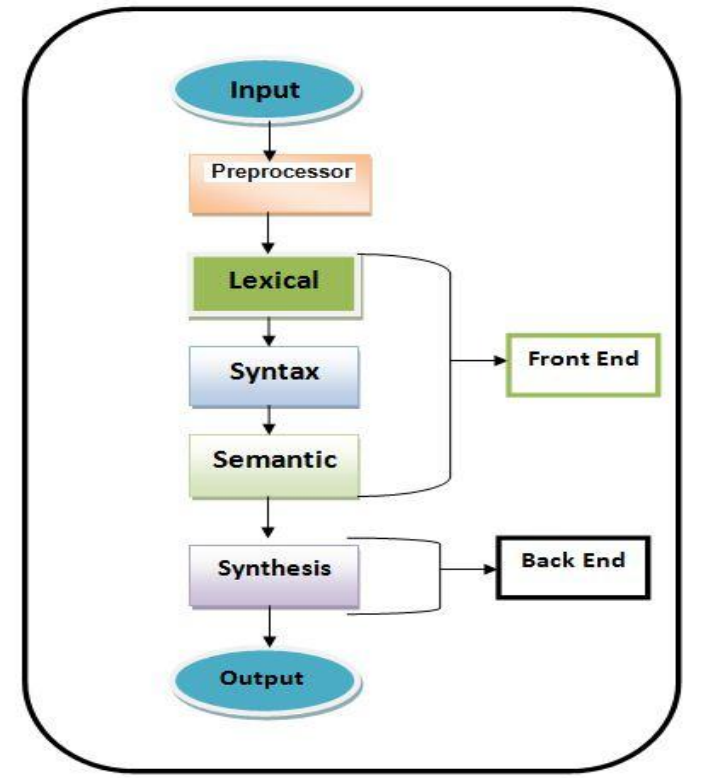
\includegraphics[width=5cm]{ch2-images/AlfEih2.png}
\caption{Alf..Eih stages of Implementation \cite{razaq2019designing}}
\label{fig:Alf..Eih stages of Implementation}
\end{figure}

The input program is first written in Arabic while adhering to the language's grammar rules. Spaces and newlines that cause issues are removed from the program after it has been written in the preprocessing step. The lexer examines the code after the preprocessing step to produce the tokens. If the component is absent, a lexical error takes place. The following stage, known as syntax, examines the input's grammatical structure to determine whether it is correct. Next comes the semantic stage, in which definitions are linked with the use and testing of each statement in terms of meaning. In the synthesis stage, the source code is translated to the equivalent C++ code, and after this stage, the code is ready to run. The following figures are examples illustrating each stage of the implementation:

\begin{figure}[H]
\centering
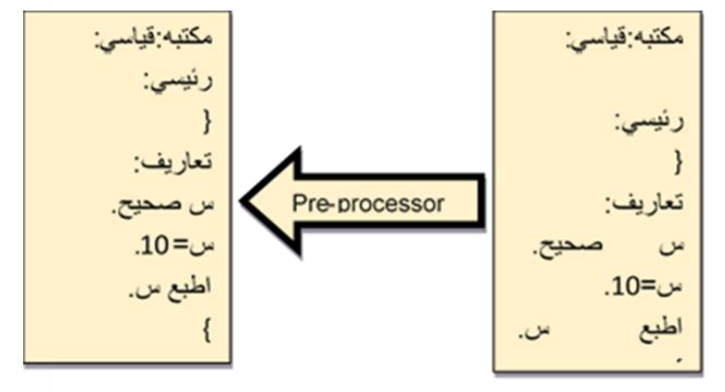
\includegraphics[width=7.5cm]{ch2-images/AlfEih3.png}
\caption{Alf..Eih Preprocessor \cite{razaq2019designing}}
\label{fig:Alf..Eih Preprocessor}
\end{figure}

\begin{figure}[H]
\centering
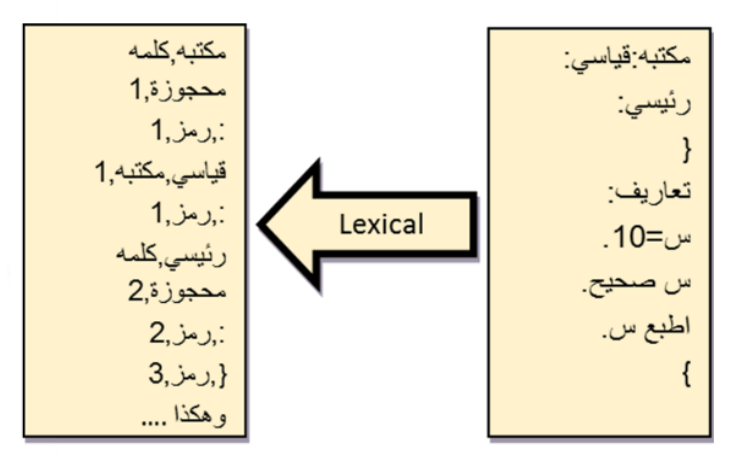
\includegraphics[width=7.5cm]{ch2-images/AlfEih4.png}
\caption{Alf..Eih Lexer \cite{razaq2019designing}}
\label{fig:Alf..Eih Lexer}
\end{figure}

\begin{figure}[H]
\centering
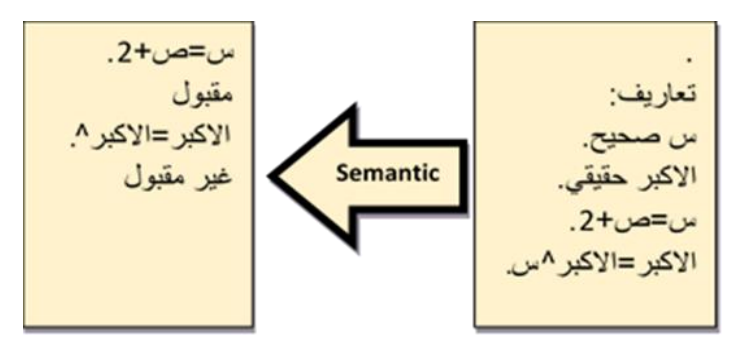
\includegraphics[width=7.5cm]{ch2-images/AlfEih5.png}
\caption{Alf..Eih Semantic \cite{razaq2019designing}}
\label{fig:Alf..Eih Semantic}
\end{figure}

\begin{figure}[H]
\centering
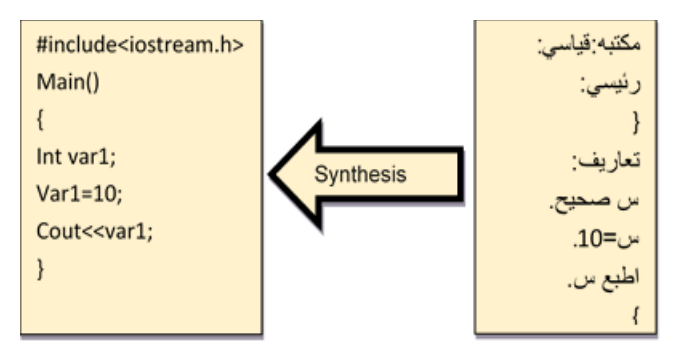
\includegraphics[width=7.5cm]{ch2-images/AlfEih6.png}
\caption{Alf..Eih Synthesis \cite{razaq2019designing}}
\label{fig:Alf..Eih Synthesis}
\end{figure}

It is recommended to put Alf..Eih in a test in schools to see its effectiveness in stimulating interest in computer programming. The language should also be expanded to include more library functions, loops, and classes ought to be added to the language. Students can better understand the ideas, guidelines, and needs of programming languages by adding Alf..Eih into the middle and high school curricula.
\subsection{Scratch}
 Dasgupta and Mako Hill \cite{dasgupta2017learning} created Scratch, a \ac{VPE}, whose primary goal is to help children learn to program. A unique source of observational data is provided by Scratch to answer questions about the effect of localization on learning due to its large user base and localization into dozens of languages. To specify the behavior of on-screen graphical objects known as sprites, programs in Scratch are created by dragging and dropping visual building blocks. In Scratch, blocks are the equivalent of tokens in text-based programming languages. They can be used in several ways, like moving a character on the screen, altering a variable, or repeating a series of instructions. The language preference is maintained between browser sessions through the use of \ac{HTTP} cookies. In the following figure, there is a Scratch code represented in four different languages:

\begin{figure}[ht]
\centering
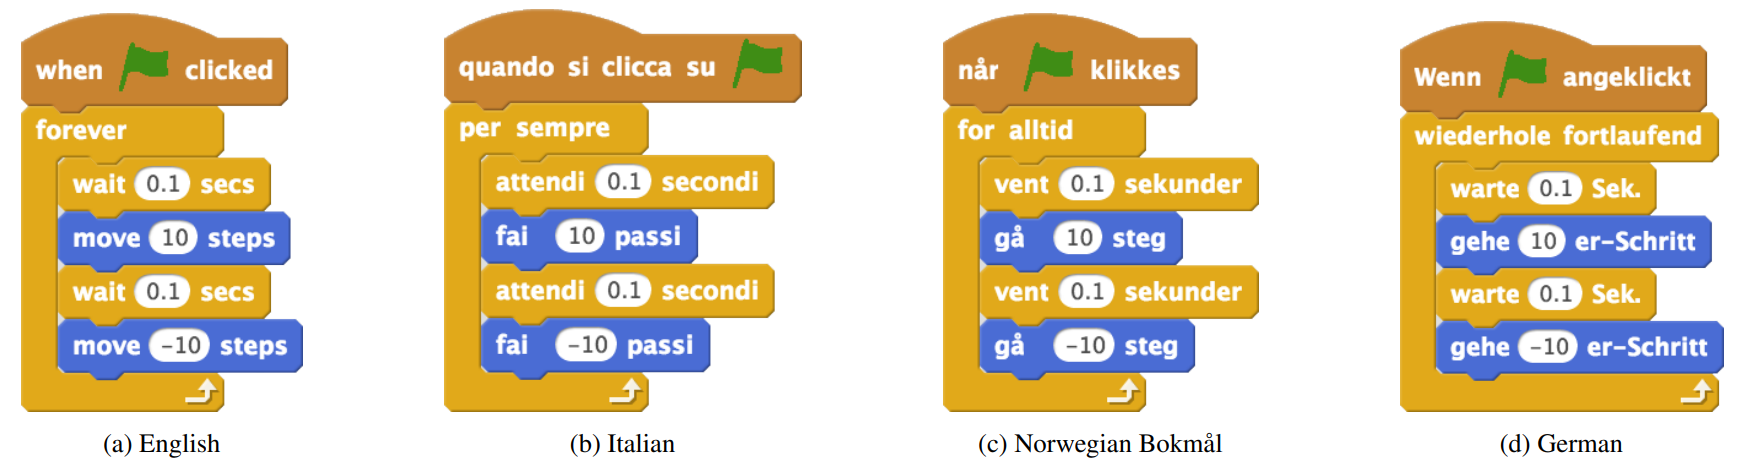
\includegraphics[width=15cm]{ch2-images/scratch.png}
\caption{Functionally Identical Scratch Code Represented in Four Different Languages \cite{dasgupta2017learning}}
\label{fig:Functionally Identical Scratch Code Represented in Four Different Languages}
\end{figure} 

Learning in Scratch is measured by the total number of blocks utilized, updated with each new project shared. This measure is used as the dependent variable in the analysis.

The study compares Italian-speaking users using Italian interfaces against those using non-localized English interfaces to determine whether people interact with Scratch using a localized interface. It is necessary to deduce each user's primary language and interface language to generate the variable using observation data. There are several reasons why someone would use Scratch in a language different than their native language. One reason is that the user could not be aware that the interface has a menu for changing languages or that there might be other technical issues.

Few languages are fully translated on Scratch because translation relies on volunteer work. Websites built with Scratch were updated frequently to correct bugs, so translations are now outdated. Because of this, the analysis will concentrate on the countries that volunteered the most in translation coverage. The authors use data on users' language preferences and primary languages to create a dummy variable indicating if a user's preferred interface language matches their home country's most widely used language. The study focuses on users from Portugal, Italy, Brazil, Germany, and Norway, and the authors conducted a similar analysis with two additional countries (France and Slovenia) as a double check. The following figure shows statistics for the usage of Scratch in different countries:

\begin{figure}[H]
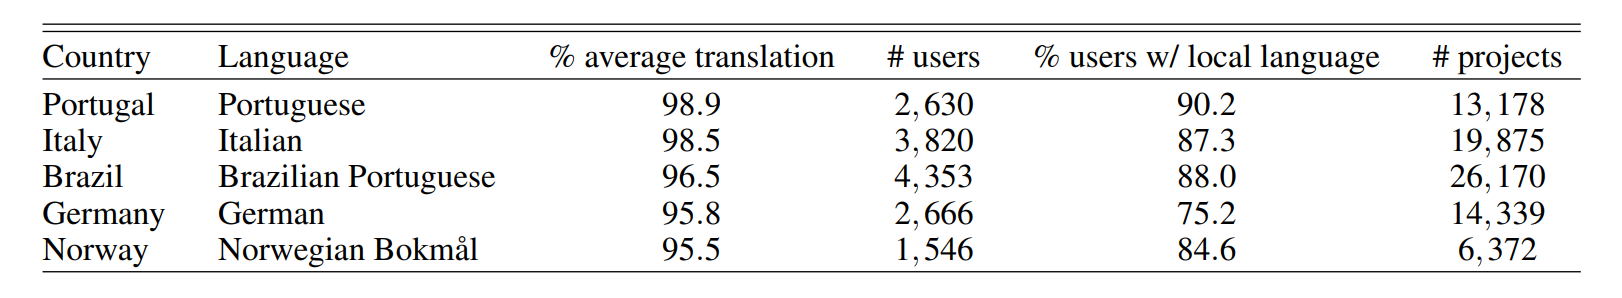
\includegraphics[width=15cm]{ch2-images/scratch2.png}
\caption{Countries included in the dataset used in this paper, along with the corresponding primary language, average translation level, number of users, proportion of users who use Scratch in the local language, and the total number of projects (with usable language data) per country \cite{dasgupta2017learning}}
\label{fig:Statistics for Usage of Scratch in Different Countries}
\end{figure} 

It is evident from the analysis and results that learners have better learning outcomes when using their language. The measurement of block repertoire has some drawbacks. One is that it can't tell whether a block is being used correctly or whether the user is aware of its purpose. To completely understand learners' comprehension, a qualitative study may be conducted.

Scratch is an excellent programming language because it offers a fully localized user interface, including programming language translations. The research supports the idea that young programmers learn faster with localized interfaces. Still, the most important effect of localization that the analysis fails to measure may be that working in the programmer's primary language encourages people who might not otherwise learn computer programming.
\subsection{Catrobat}
Awwad \cite{awwad2017localization} created Catrobat, a VPE similar to Scratch. The version of Catrobat, developed for Android smartphones, is named Catroid \cite{slany2012mobile} and is available on Google’s Play Store as ``Pocket Code”. It is a learning application that allows children and young people to create their own games, animations, and interactive apps on their phones or tablets using a VPE. Many countries promote programming education for primary and secondary school children, with VPEs typically used to teach programming. However, the release of VPEs worldwide requires the internationalization and localization of the product, particularly for bidirectional languages like Arabic, Persian, and Urdu. 

Many complex issues of bidirectional software localization remain unaddressed, preventing it from reaching its full potential. The Catrobat VPE has been localized into bidirectional and specifically to the Arabic language to address the difficulties that application developers confront. The localized VPE meets bidirectional requirements, complies with bidirectionality design guidelines, and can be used in programming education for young schoolchildren.

Internationalization and localization are crucial for software to be used in several locations. Internationalization refers to the process of re-engineering a system to support many languages and regions. In contrast, localization refers to the process of modifying an internationalized piece of software for use in a particular nation or culture by including locally relevant features and translated text. Due to its built-in support for localization components, an application that has been successfully internationalized is simpler to localize. Three key steps must be taken for localization to be successful: translating all text the user sees, adapting images and user interface components for diverse cultural contexts, and adding a locale to ensure that regional formats are presented correctly. The following figure shows the process of internationalization and localization:

\begin{figure}[H]
\centering
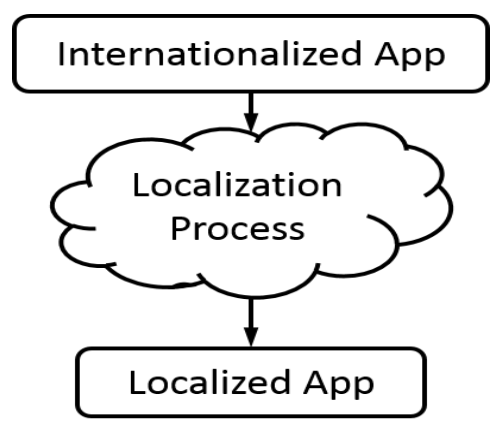
\includegraphics[width=7.5cm]{ch2-images/catrobat.png}
\caption{The Localization Process \cite{awwad2017localization}}
\label{fig:The Localization Process}
\end{figure} 

There were numerous difficulties encountered while attempting to localize Catrobat into bidirectional languages. However, solutions for establishing a dependable right-to-left user interface were offered. Arabic text and other complex scripts require unique rendering due to various script characteristics such as bidirectional text, contextual shaping, character reordering, and linking. Pocket Code has trouble with complex scripts, even if it can show many European languages. A program that displays text on the program's stage was developed to address this problem. Complex scripts cannot, however, be displayed using the bitmap font technology used by Pocket Code. The characters must first be saved in a buffer and then presented as a group for a bidirectional text to be rendered correctly. The bitmap image containing the text must be converted into a texture object to support complex bitmap font rendering for scripts such as Arabic, Urdu, and Persian. When the smartphone is set to Arabic, Pocket Code correctly displays the text with the proper directionality. The following figure shows a screenshot for the set and shows variable bricks with English and Arabic strings:

\begin{figure}[H]
\centering
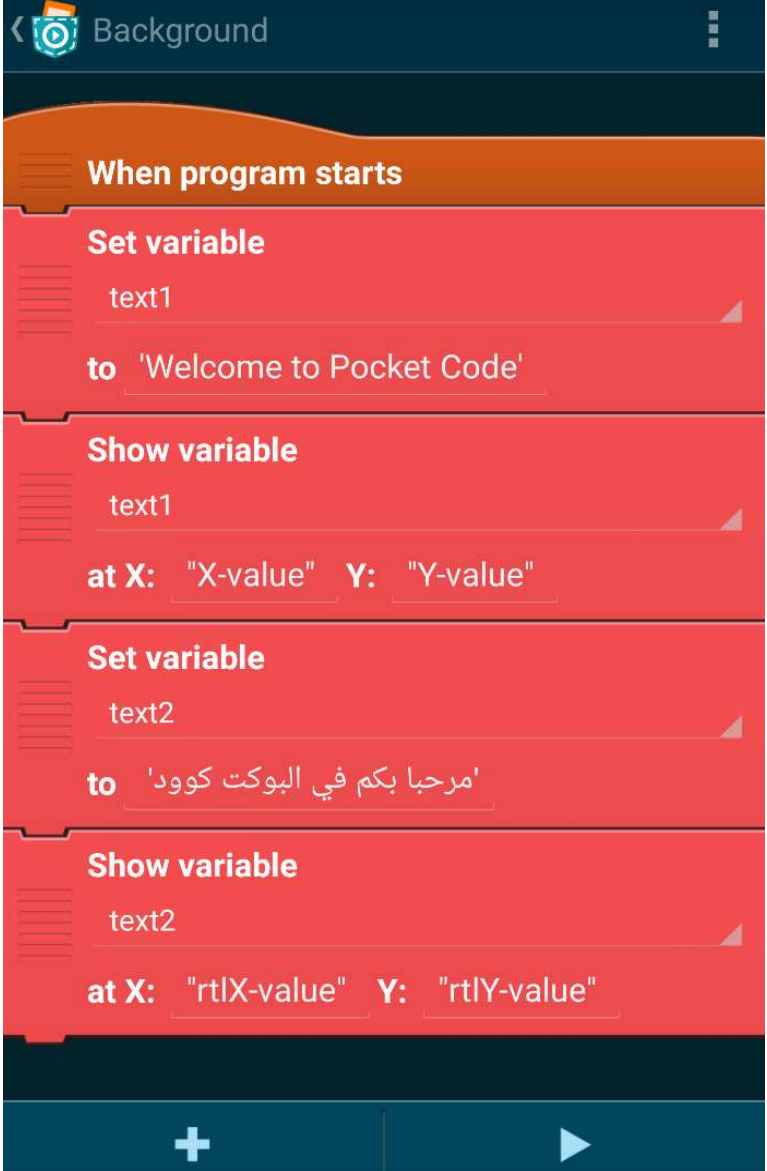
\includegraphics[width=7.5cm]{ch2-images/catrobat2.png}
\caption{Screenshot for the set and show variable bricks with English and Arabic strings \cite{awwad2017localization}}
\label{fig:Screenshot for the set and show variable bricks with English and Arabic strings}
\end{figure} 

Many challenges were faced in localizing a VPE for smartphones into bidirectional languages, specifically Arabic. The localization process involves adapting the software to suit the new culture and changing the source code and icons. The localization testing showed that Catrobat met bidirectional requirements that comply with bidirectionality design guidelines. 
\section{Summary}
To sum up, programming paradigms are one of the main aspects that must be considered while designing a programming language. To design a programming language, several tools are required to create the language: the lexer, parser, static analyzer, code optimizer, and code generator. Eclipse is one of the famous IDEs for writing and editing source code, especially for Java. Many attempts were made to design a localized programming language. Phoenix, ARABLAN, DHAD, and Alf..Eih were attempts made to create an Arabic programming language. Phoenix was the localized version of C\#, ARABLAN was the localized version of Pascal, DHAD was converted to machine code, C, assembly, while Alf..Eih was the localized version of C++. Moreover, Babylscript was a multilingual version of JavaScript, enabling users to write programmers in different languages. Finally, Scratch and Catrobat were VPEs created mainly for children to help them learn to program. 

\chapter{Design and Implementation}
\section{Project Goals}
The goal of our project is to allow programmers, especially children, to write programs using their own native language. Additionally, another goal is to create a user interface that allows users to customize the translations for their specific needs. This will be especially beneficial for teachers who are teaching programming to students who speak a variety of languages. By allowing users to customize the translations, the system will be more effective at helping students learn programming in their native language and even their dialects. Thus, an Egyptian student can write a program in Arabic and a German student can write a program in German. A non-functional goal is to make the translation process seamless by automatically adding the necessary project configurations without requiring the user to know the implementation details.
\section{Project Overview}
I will be creating an Eclipse Plugin that localizes source code. Using this plugin, a user (for example a teacher) will be able to define Java keywords, \ac{API} identifiers like class names, method names, and exception messages in their own native language. Moreover, the Eclipse Plugin can convert an existing Java file to the user's chosen language. Also, the Eclipse Plugin has commands to update the project's configurations with the necessary compile time and runtime components. At compile time, Maven, which is the build automation tool used to build the program, performs transpilation from the localized language to Java. In runtime, there is a component that translates the exception messages that occur at runtime. The source code of this project is available on the following GitHub repository https://github.com/omar-elmeteny/Thesis.
\section{Design Approach}
The design approach follows a modular structure where each component focuses on a specific task and can be independently developed and tested. The components interact with each other to ensure a seamless flow of translation and transpilation processes.

By implementing this design approach, the project can achieve the goal of localizing the Java programming language, allowing developers to write code in their native language and automatically transpiling it to Java during the build process. The Java ecosystem has several choices of tools to automate the build, such as ANT, Maven, and Gradle. I chose to initially support Maven.

I also chose not to make any changes to the semantics and basic syntax of the Java programming language. The code written in a native language is basically a one-to-one translation of the keywords and identifiers without new grammar rules or changes to the rules of the Java Programming language.

The project consists of several components and packages that work together with the Maven build automation to achieve the desired functionality. The implementation details of these components will be explained in the following section. The following diagram shows the components and how they interact with each other:

\begin{figure}[h]
\centering
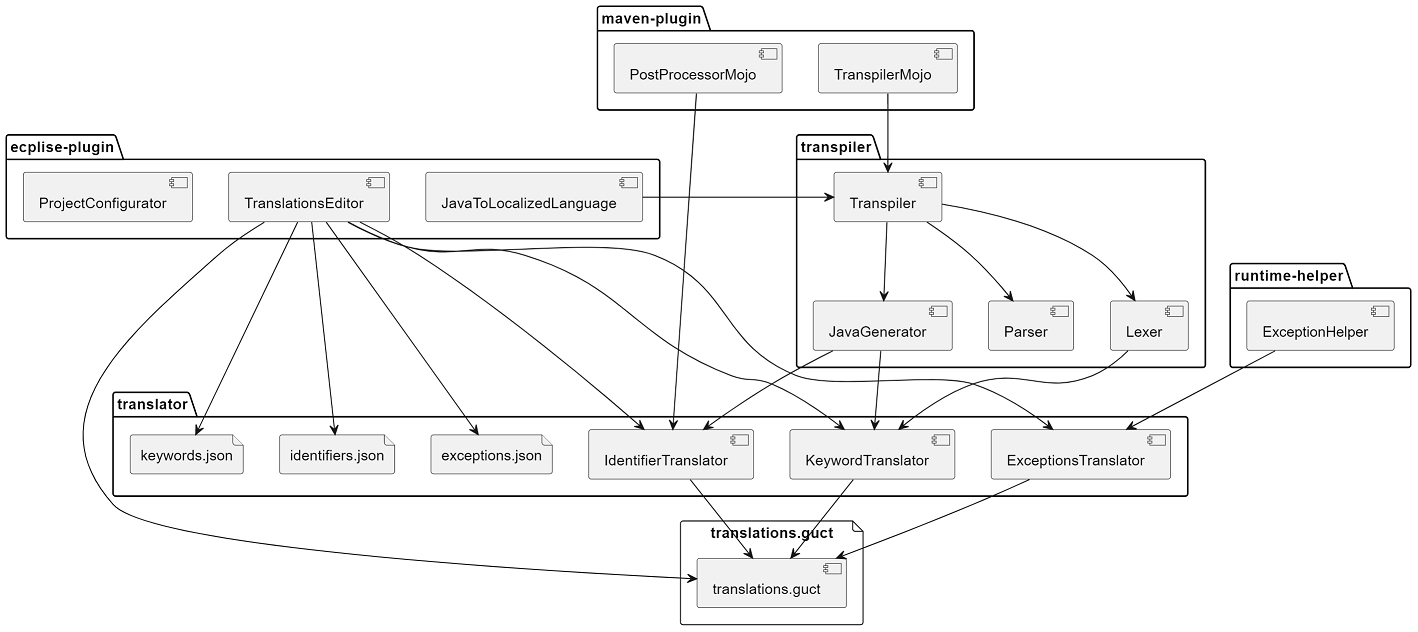
\includegraphics[width=15cm]{ch3-images/components.png}
\caption{Project Components}
\label{fig:Project Components}
\end{figure} 

\section{Implementation Details}
\subsection{Eclipse Plugin}
This plugin adds support for language localization to the Eclipse IDE. 

\subsubsection{Third Party packages}
\begin{enumerate}
    \item \textbf{org.apache.maven.maven-model}: This is a library used to read, parse, and edit the pom.xml file of the user's project.
\end{enumerate}
\subsubsection{Java to Localized Language Command}
This command is added as a context menu item of the project's menu to allow the user to convert an existing Java file or all Java files in a project or a folder depending on the user's selection to a .guc file (or files) depending on the project's default source language. After converting, the java file is backed up to ``.java.bak" and deleted because it can conflict with the generated .guc file during compilation. 

\begin{figure}[H]
\centering
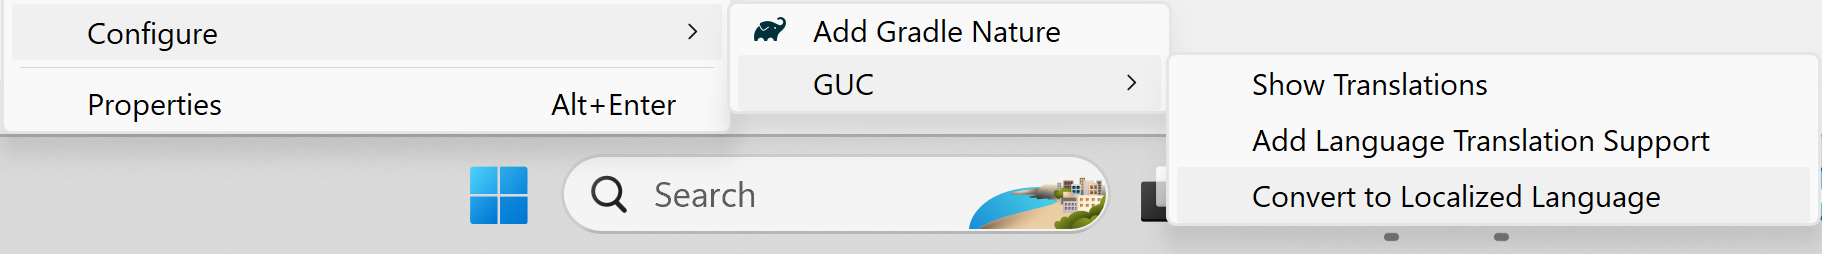
\includegraphics[width=15cm]{ch3-images/eclipsecontextmenu.png}
\caption{Additions to the project's context menu}
\label{fig:Additions to the project's context menu}
\end{figure} 

\subsubsection{Language Translation Support Command}
This command is added as a context menu item of the project's menu to add support for language translation to an existing Maven project. Refer to figure \ref{fig:Additions to the project's context menu} to see the command in the project's context menu. It does so by adding the following changes to the project's pom.xml file:

\begin{enumerate}
    \item Add the repository https://maven.languageslocalization.com/snapshots to both the plugin repositories and repositories. This Maven repository contains my dependencies so that Maven can download the required libraries.
    \item Add the translations.guct as a resource in the output jar file for the project so it could be read by the Runtime Helper package (which will be discussed later) during runtime to perform exceptions translation.
    \item Add the Runtime Helper package as a dependency for the project which is used to translate exceptions in runtime. By referencing this library, all the other needed packages such as the Translator package are included in the project by being indirectly referenced.
    \item Add the build-helper-maven-plugin to make sure that the generated .java files are included in the build.
    \item Add the Transpiler Maven Plugin package to transpile the .guc files and process the .class files after compilation (which will be explained later).
\end{enumerate}

\subsubsection{Translations Editor}
This editor is used to translate keywords, identifiers, and exceptions and saves these translations in the translations.guct file. The editor can be opened by pressing ctrl+G or using the command added in the project menu (see to figure \ref{fig:Additions to the project's context menu}). The translation.guct file has the extension .guct to be a content type to be able to create the user interface for the file. This editor is a Multi-page Editor which consists of five pages:

\begin{enumerate}
    \item \textbf{Keywords Page}: This page is used to translate Java keywords to any target language chosen by the user. The keywords and their translations are represented in a table where the left column is the keyword and the right column is the translation. There is a drop-down menu to select the target language. There is also a button to add default translations without changing the translation already edited by the user, which is disabled if there are no translations to a certain target language. The editor calls the Keyword Translator component (which will be discussed later) to read and write the translations. The following figure shows the Keywords Page in Eclipse:
   
    \begin{figure}[H]
    \centering
    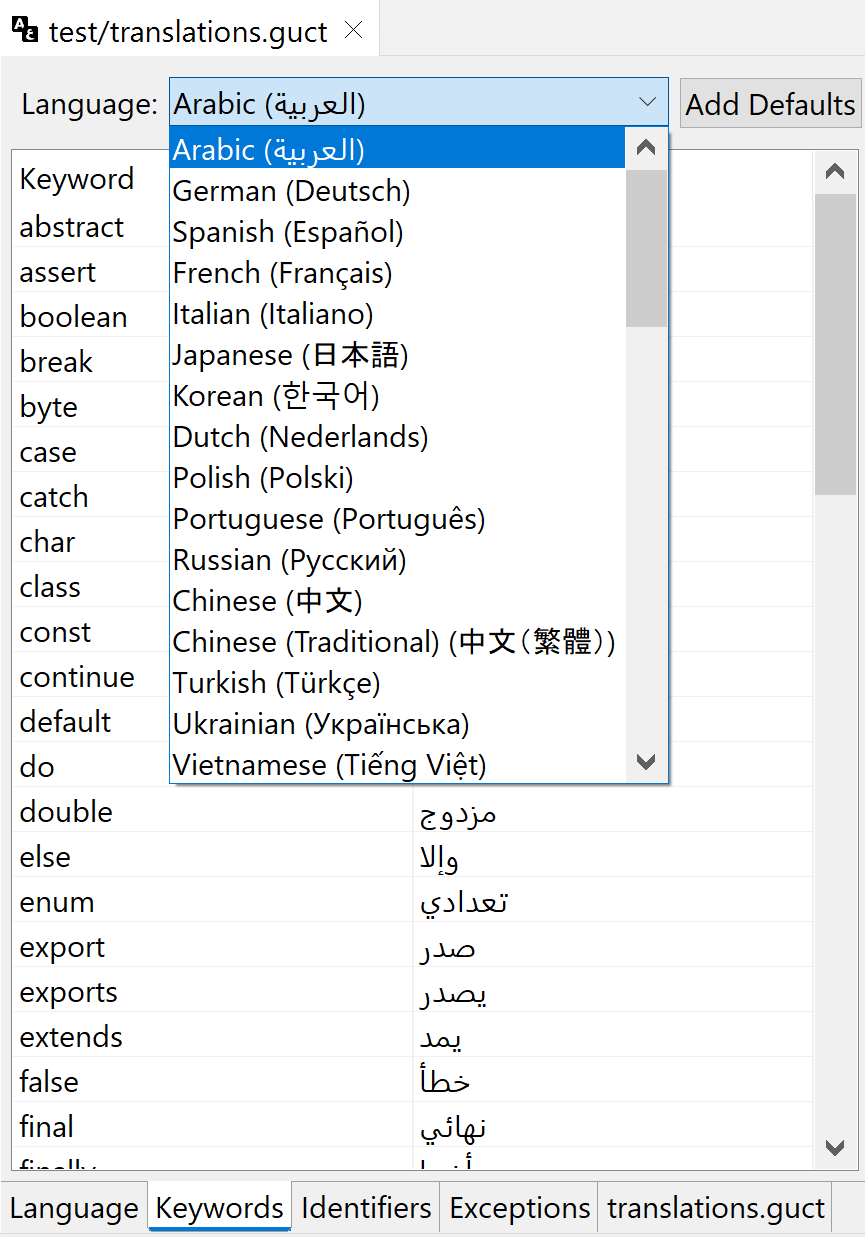
\includegraphics[height=9cm]{ch3-images/keywordspage.png}
    \caption{Translations Editor: Keywords Page}
    \label{fig:Translations Editor: Keywords Page}
    \end{figure}
    
    \item \textbf{Identifiers Page}: This page is used to translate identifiers to any target language chosen by the user. This page is similar to the Keywords Page but has some differences. The identifiers and their translations are represented in a tree instead of a table because Java has many identifiers. This tree is created by traversing the src.zip file found in the Java home folder. Moreover, there is a search bar to search for a specific identifier. Searching can be case-sensitive or exact match or both of them. Translations are performed by calling the Identifier Translator component (which will be discussed later). The following figure shows the Identifiers Page in Eclipse:

    \begin{figure}[H]
    \centering
    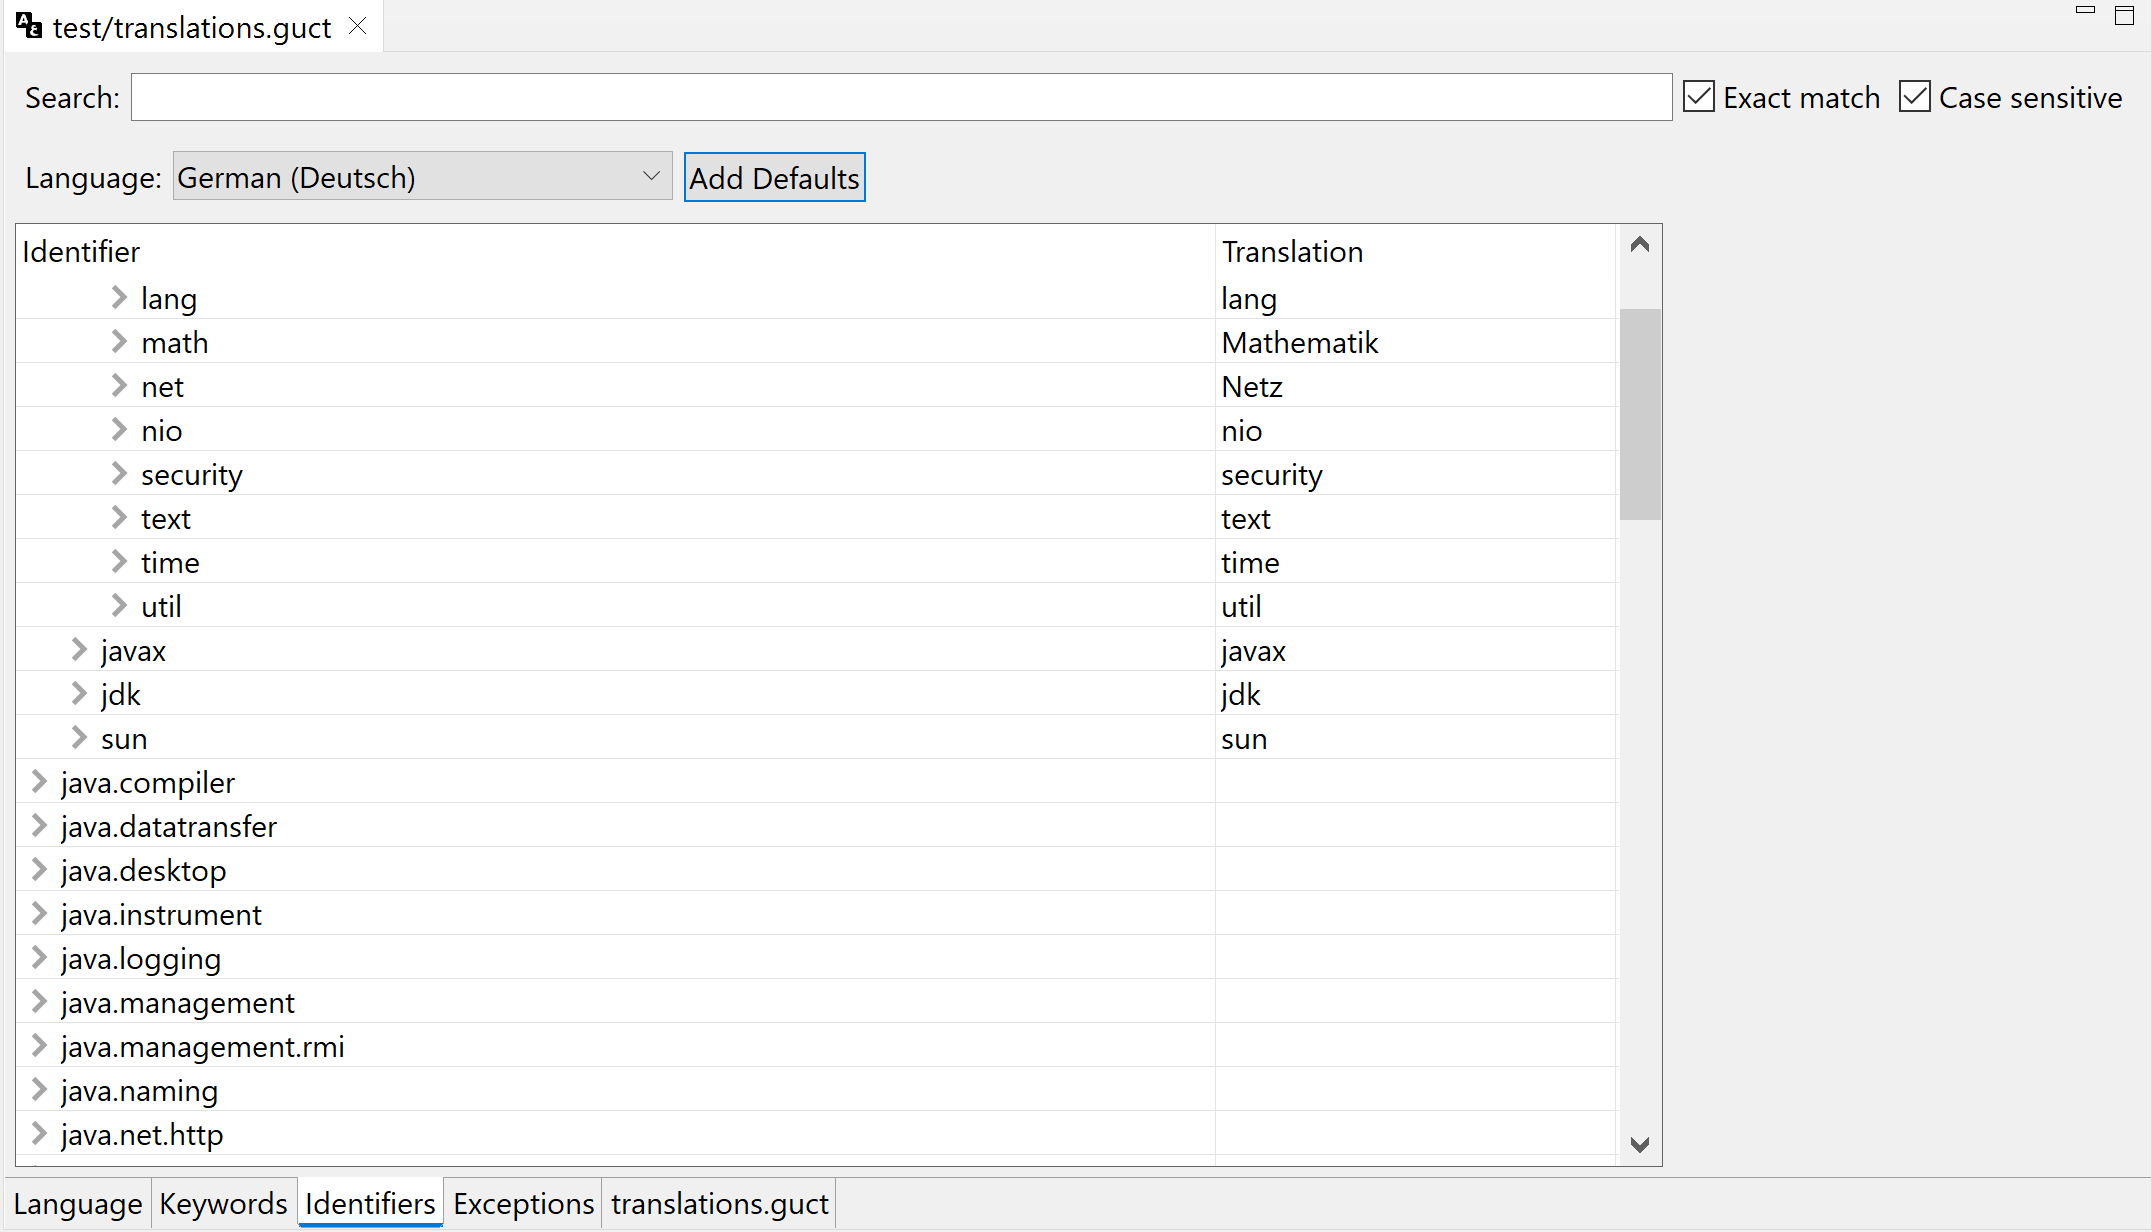
\includegraphics[width=15cm, height=10cm]{ch3-images/identifierspage.png}
    \caption{Translations Editor: Identifiers Page}
    \label{fig:Translations Editor: Identifiers Page}
    \end{figure}
    
    \item \textbf{Exceptions Page}: This page is used to translate exceptions. It is similar to the Identifiers Page but with some differences. One difference is that the tree represents the classes that inherit from the class Throwable instead of representing all classes, methods, and fields. One of the challenges, relating to runtime exception messages translation, is that the message usually includes information that helps the user identify what went wrong. For example, the message "Index 15 out of bounds for length 10" has two pieces of information that can help the user fix the problem. The first is the array index 15, and the second is the array of length 10. The translator extracts those values using Regular Expressions and includes them in the translated message, as explained in this section and later in more detail in the Translations File section. To achieve this, the tree has three columns instead of two. One for the exception names, one for the regex (Regular Expression), and one for the translation of the exception's message. The regex field must be written in English. When a user writes in the regex column, a message is automatically written in the translations field in English, which is a copy of the regex statement except that the capture groups are replaced (which will be discussed later in detail). To translate to another language like Arabic, the user must edit the automatically generated message to Arabic, leaving the symbols replaced with the capture groups. The user can write more than one regex for the same exception, so when they enter a regex statement, another row for the same exception is created. To delete a regex statement, the message must be deleted. The user can also write a message without a regex if the exception doesn't need a regex. The translations are added to the translation.guct file when the user saves all their changes. Note that if the user didn't enter a translation without a regex, a default translation would be automatically written in the translations.guct file (i.e. the default translation will be English (Java)). The following figure shows the Exceptions Page in Eclipse:

    \begin{figure}[H]
    \centering
    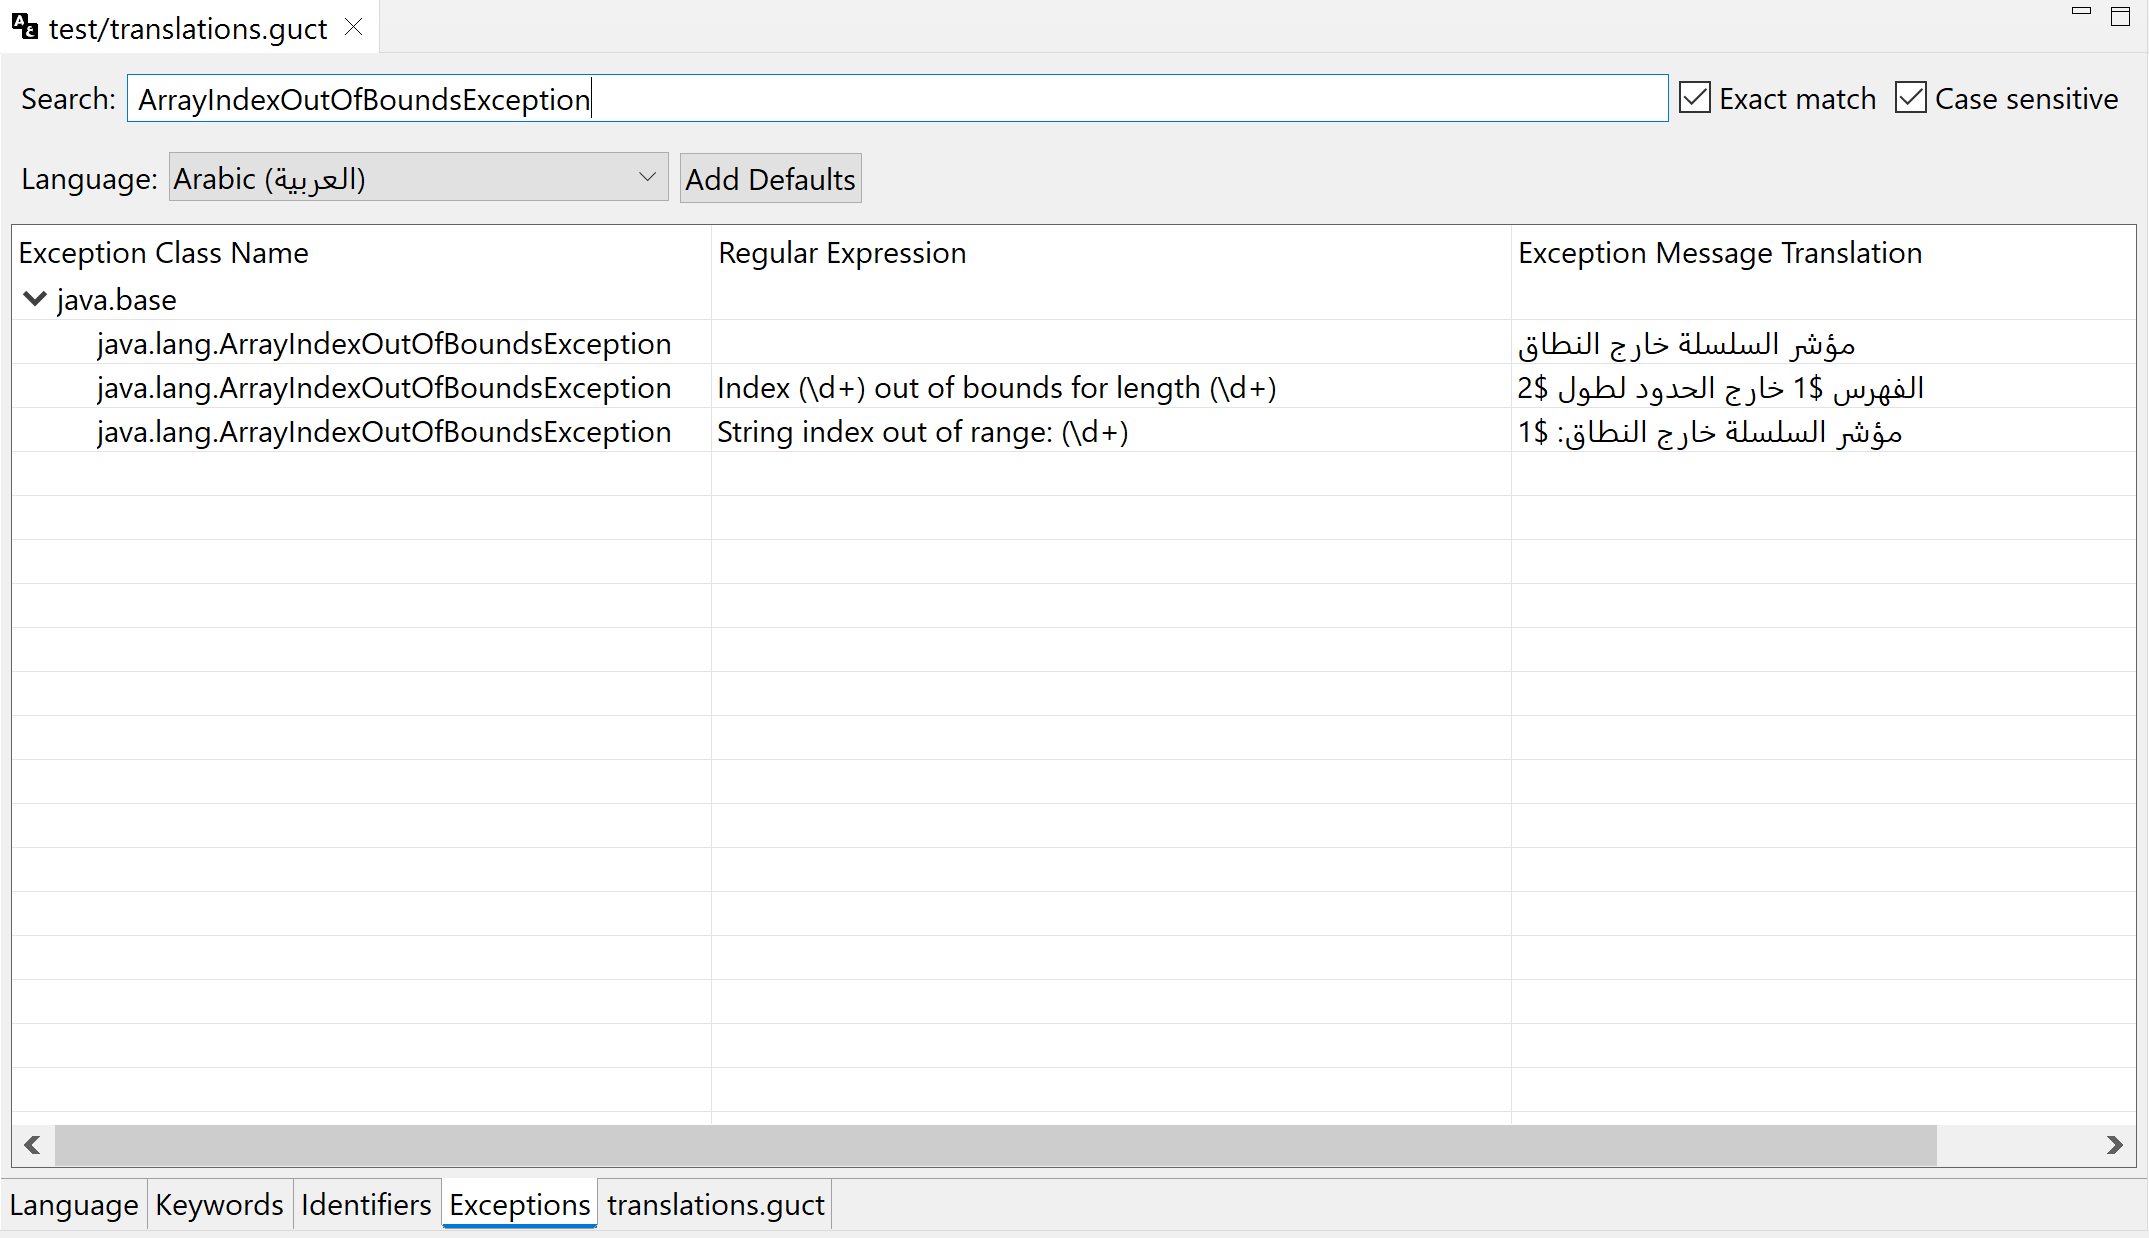
\includegraphics[width=15cm, height=10cm]{ch3-images/exceptionspage.png}
    \caption{Translations Editor: Exceptions Page}
    \label{fig:Translations Editor: Exceptions Page}
    \end{figure}

    
    \item \textbf{Project Language Page}: On this page, the user can change the default language of the project. The default language is initially set to Arabic. Languages are represented in a drop-down menu. The following figure shows the Project Language Page in Eclipse:
    
    \begin{figure}[H]
    \centering
    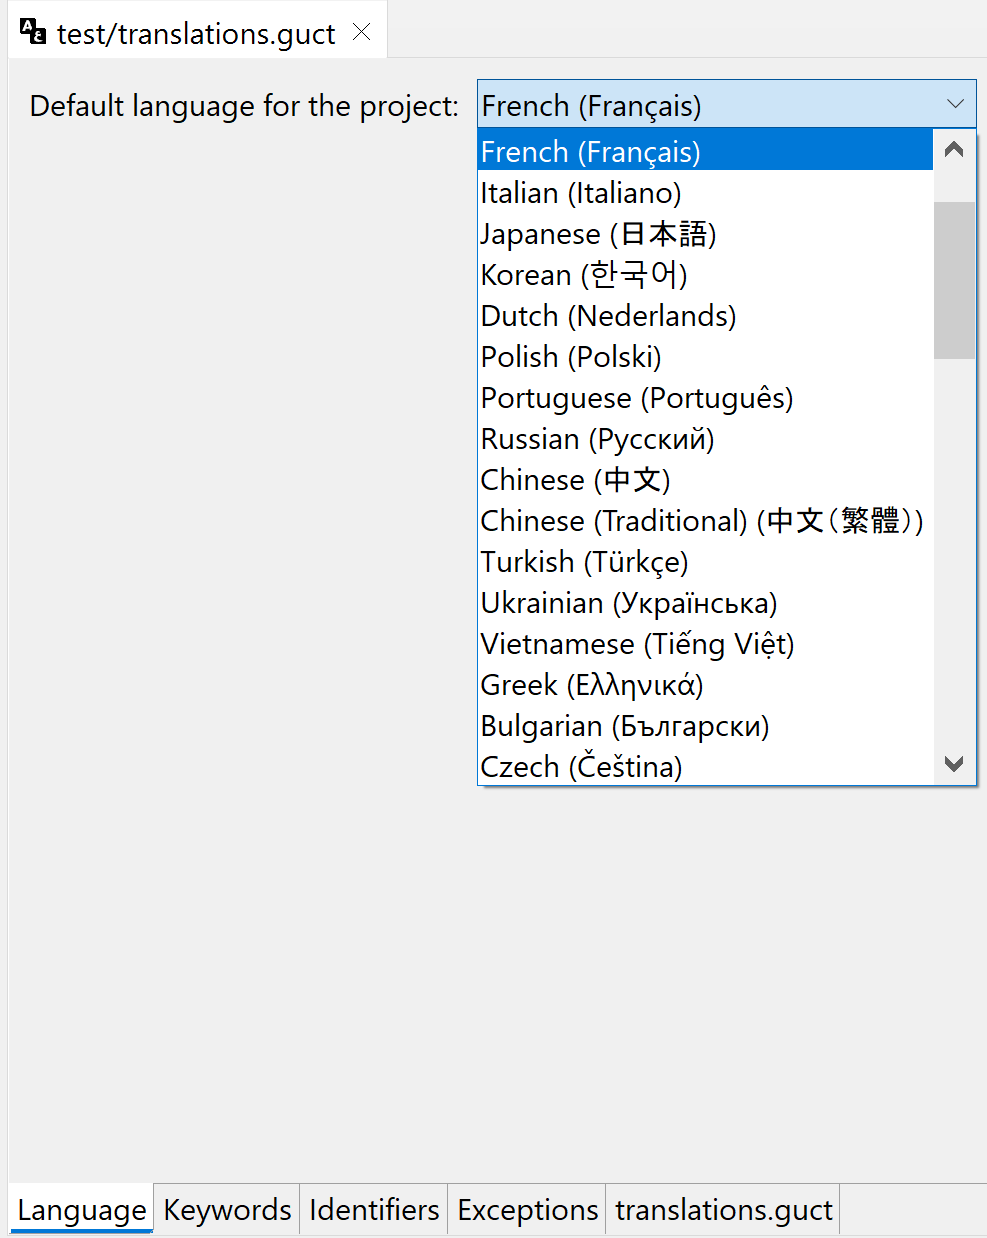
\includegraphics[width=10cm, height=10cm]{ch3-images/defaultlanguage.png}
    \caption{Translations Editor: Project Language Page}
    \label{fig:Translations Editor: Project Language Page}
    \end{figure}

    \item \textbf{translations.guct}: This page is used to translate keywords, identifiers, and exceptions and change the project language by editing the JSON directly. This makes it easier for the user to add translations if they have a JSON file filled with translations. The updates done to JSON are reflected in the user interface of the other pages and vice versa.

\end{enumerate}

\subsubsection{Source-code Editor}
This editor is used to write the programs based on the chosen project language. It has only one page, and the file has an extension ``.guc" to be a content type in Eclipse. The editor supports bidirectional languages like Arabic, Urdu, and Persian. The following figures show the Bubble Sort algorithm in Java and its equivalent Arabic code after using the ``Convert to Localized Language" command (see figure \ref{fig:Additions to the project's context menu}): 

    \begin{figure}[H]
    \centering
    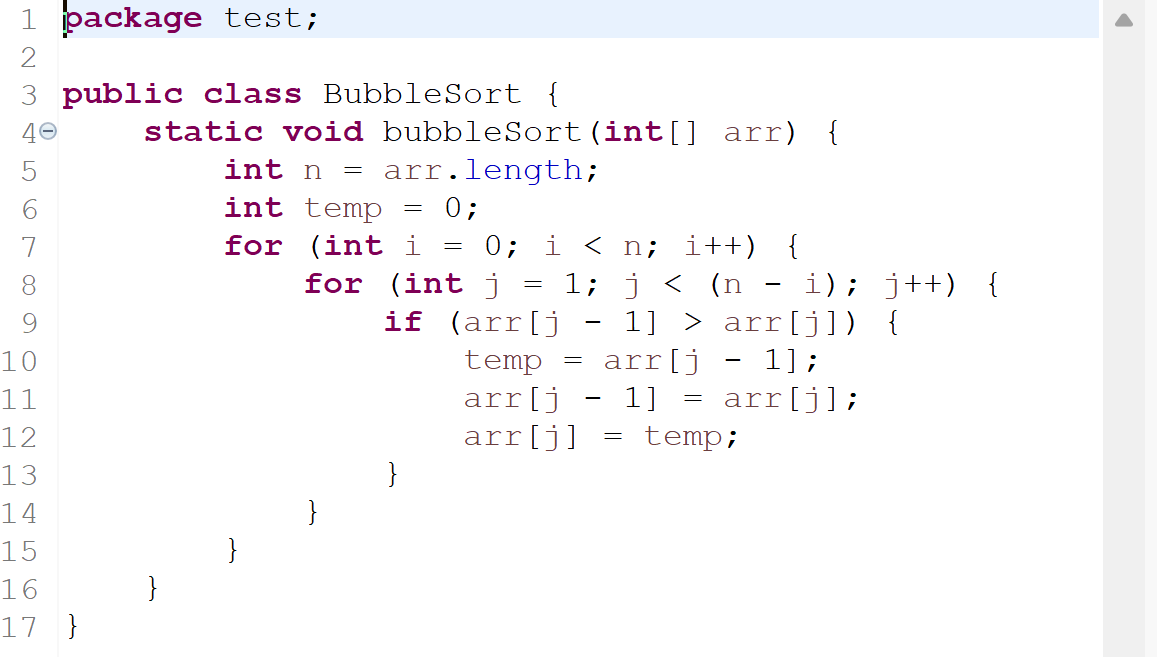
\includegraphics[width=6.5cm]{ch3-images/bubblesort.png}
    \caption{Bubble Sort Algorithm in Java}
    \label{fig:Bubble Sort Algorithm in Java}
    \end{figure}

    \begin{figure}[H]
    \centering
    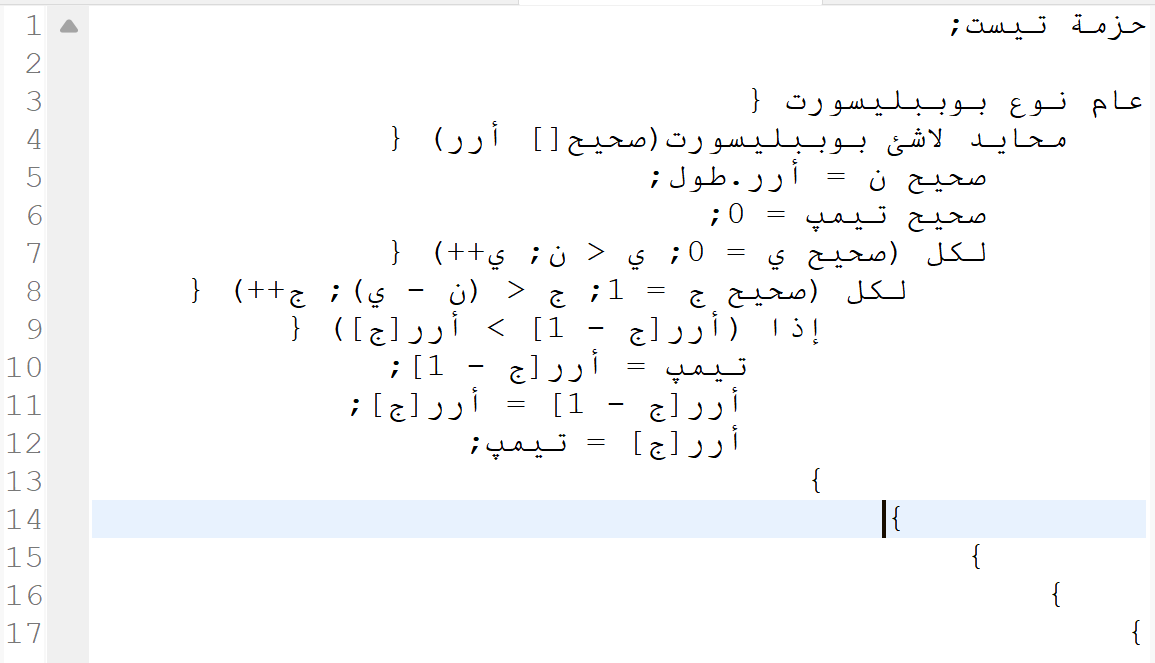
\includegraphics[width=6.5cm]{ch3-images/bubblesort_ar.png}
    \caption{Bubble Sort Algorithm in Arabic}
    \label{fig:Bubble Sort Algorithm in Arabic}
    \end{figure}

The bidirectional support is obvious in the above figure (figure \ref{fig:Bubble Sort Algorithm in Arabic}). In the Transpiler section (which will be discussed later), how the Java code is generated will be explained, taking the Arabic Bubble Sort algorithm as an example.

\subsection{Translations File}
The translations.guct file is one of the main components of the project because its acts like a database in saving information related to translations. The translations.guct file has a structure that is exactly similar to the structure of a JSON file. 

The translation.guct file consists of a JSON object consisting of four keys: defaultLanguage, keywords, identifier, and exceptions. The defaultLanguage key has a value corresponding to the native language that the user will use in their project. This value is the ISO 639-1 of the language name. For example, if the default language is Arabic, then the value will be "ar" and if the user chooses German, then the value will be "de" and so on. The defaultLanguage is initially set to ``ar"" (Arabic) because this project is done in Egypt.

The following key is the keywords key which is a JSON object whose keys are all Java keywords, and values are objects where the key is the ISO 639-1 language name to which the Java keyword is translated and the value is the translation of the keyword. 

The next key is the identifiers and it has exactly the same structure of keywords. Note that if a keyword or identifier is not found, then its translation to any language will be the keyword or the identifier itself. Moreover, when I have a full class name or a package name such as "java.lang.String", it is treated as three separate identifiers java, lang, and String.

The last key is the exceptions key and it includes another object where the key is the full class name of the exception (e.g. java.lang.ArrayIndexOutOfBoundsException) and the value is an array of objects. This array includes one or more objects because an exception may have more than one error message format where each object consists of two keys: regex and messages. The regex (Regular Expression) key is included in the object because some error messages are not static but dynamic. The regular expression is used to determine whether the exception message matches a specific message format in which case the parameters for the message are captured in capture groups, and these groups are used in the string replacement when the message is translated. For example, the error message of ArrayIndexOutOfBoundsException in Java can change depending on the specific context in which the exception is thrown. This exception is generally thrown when a program attempts to access an array element using an index that is out of bounds. For example, if an array has five elements, but a program tries to access the sixth element, then an ArrayIndexOutOfBoundsException will be thrown. The error message displayed when this exception occurs in Java will typically include information about the array that caused the exception, as well as the index that was out of bounds. For example, the error message might look something like this:
\begin{lstlisting}[language=java]
Exception in thread "main" java.lang.ArrayIndexOutOfBoundsException: Index 6 out of bounds for length 5
    at MyClass.myMethod(MyClass.java:25)
    at MyClass.main(MyClass.java:10)

\end{lstlisting}


The regex value should be "Index (\textbackslash{\textbackslash{d+}}) out of bounds for length (\textbackslash{\textbackslash{d+}})" because the 6 and the 5 can be other numbers in other cases. The messages key is the other key in the object and it includes another object which is the ISO 639-1 language name to which the Java keyword is translated and the value is the translation of the keyword. In this example, the translation should include \$1 and \$2 which are replaced by the values of the corresponding capture groups. Note that the regex is an optional key and mustn't be included in the object if the error message is not dynamic. When the regular expression is omitted, the corresponding translation is used when none of the regular expressions match the exception message.

Here is a simple example of a JSON object that could be written in the translations.guct file: 

\begin{figure}[H]
\centering
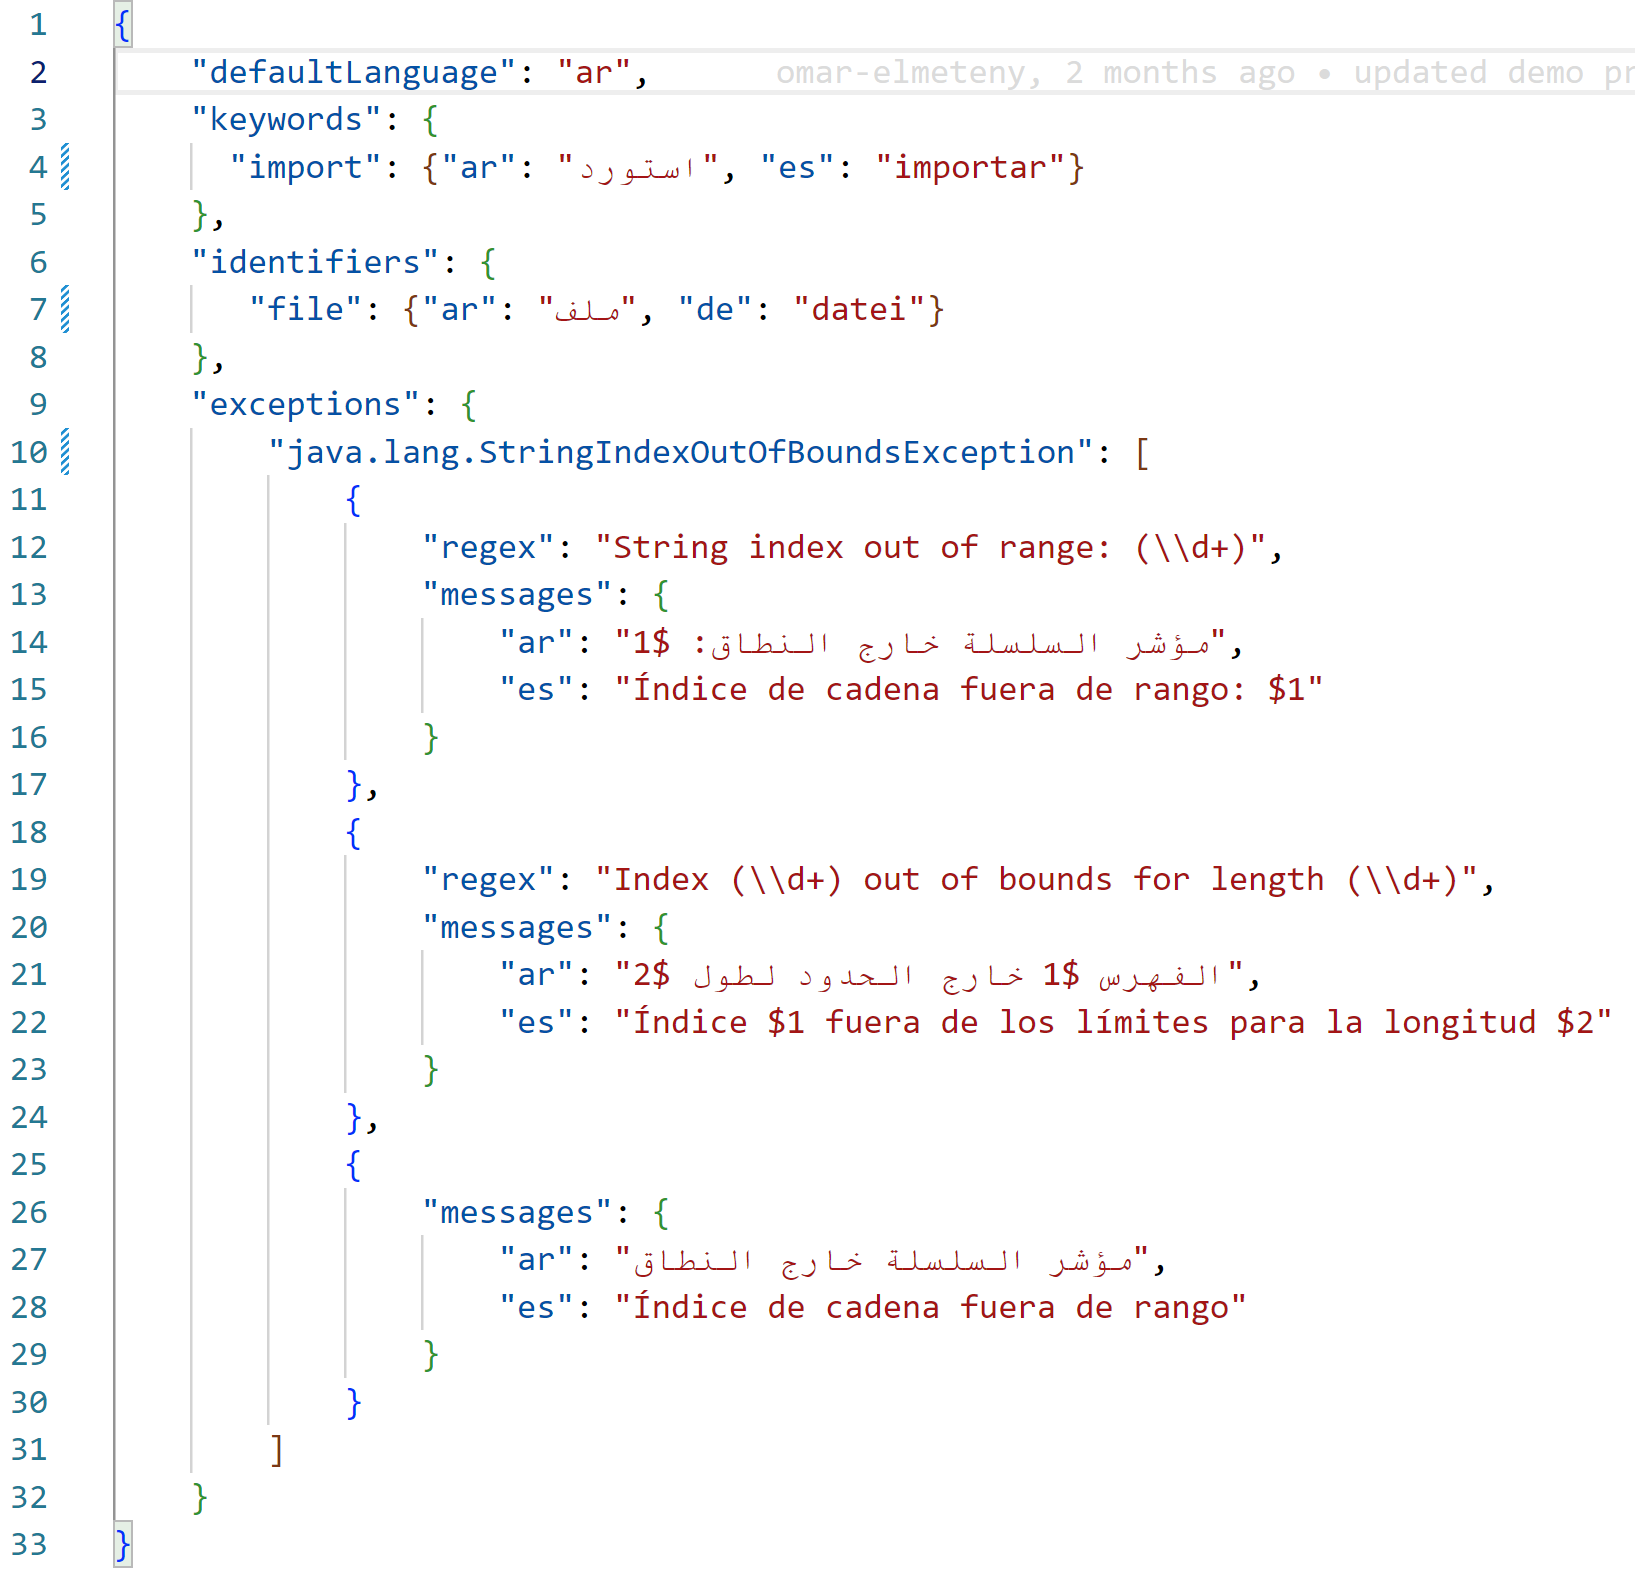
\includegraphics[width=12.5cm]{ch3-images/translationsfile.png}
\caption{An example of a translation.guct file}
\label{fig:An example of a translation.guct file}
\end{figure} 

\subsection{Translator Package}
The Translator package is responsible for translating keywords, identifiers, and exceptions from the source language to English and vice versa. This is done by reading the JSON file.
\subsubsection{Third Party packages}
The Translator package uses three third-party packages:
\begin{enumerate}
    \item \textbf{org.json}: A package for parsing and writing JSON format.
    \item \textbf{com.ibm.icu.icu4j}: A package to transliterate text using non-ASCII letters to ASCII letters. For example ``\<زر>" is transliterated to ``zr".
    \item \textbf{commons-io}: Used to handle files containing Unicode Byte Order Marks (BOM).
\end{enumerate}

\subsubsection{Resource Files}
The Translator package contains three JSON files including default translations for keywords, identifiers, and exceptions. The translations don't cover all languages but only five languages: Arabic, French, German, Italian, and Spanish because these are the most commonly spoken languages.
\begin{enumerate}
    \item \textbf{keywords.json}: This file contains the default translations for all Java keywords.
    \item \textbf{identifiers.json}: This file contains the default translations for Java's most commonly used identifiers (e.g. String).
    \item \textbf{exceptions.json}: This file contains the default translations for Java's most commonly thrown exceptions (e.g. ArrayIndexOutOfBoundsException).
\end{enumerate}
Note that the structure of each file is exactly similar to its corresponding key in the translations.guct file.

\subsubsection{Keyword Translator}
The Keyword Translator is responsible for loading the keyword translations from JSON format (see translations.guct above) to memory. It is used in translating a keyword from Java to a target language and from a source language to Java. Moreover, it is used to determine whether a particular keyword has a translation to any native language or not. It also has an API to add/change keyword translations used by the Eclipse Plugin for editing translations (as discussed earlier). The Keyword Translator can convert the data back to JSON to be saved to the project's translations.guct file.
\subsubsection{Identifier Translator}
The Identifier Translator works in a similar manner to the Keyword Translator. However, the difference is that if an identifier doesn't have a translation to the target language and both source and target languages use different scripts (e.g. Arabic and Latin), the Identifier Translator will transliterate the identifier to the target language's script (e.g. ``\<زر>" is transliterated to ``zr").
\subsubsection{Exception Translator}
The Exception Translator is used to translate exception messages and other identifiers that appear in the stack trace. It uses the Identifier Translator to translate the identifiers that appear in the stack trace. The Exception translator works only at runtime because this is when the exceptions are thrown.
\subsection{Runtime Helper Package}
This package has helper methods that are called by the generated Java code during runtime. 
\subsubsection{Third Party packages}
\begin{enumerate}
    \item \textbf{org.ow2.asm}: This library reads the .class files which are executed by the \ac{JVM} to read information about the identifiers that were translated during the transpilation process.
\end{enumerate}
\subsubsection{Exception Helper}
This component performs the task of translating the exception messages and the stack trace of the thrown exceptions. It uses the Exception Translator component in the Translator package to perform these tasks. It reads the translations.guct file during runtime (via the Translator package) and also reads the information about the identifiers that were translated during the transpilation process. This information is written in the class file by the PostProcessorMojo component (which will be explained later).
\subsection{Transpiler Package}
This package performs the actual transpilation of code from the source language to Java and vice versa. 
\subsubsection{Third Party packages}
\begin{enumerate}
    \item \textbf{org.antlr.antlr4-runtime}: \ac{ANTLR} \cite{antlr} is a powerful parser generator for reading, processing, executing, or translating structured text or binary files. This package provides the core functionality for the lexer and parser.
    \item \textbf{antlr/grammars-v4}: This is an open source repository containing ANTLR4 grammar files for many programming languages including Java. I used the Java9 grammar files from this repository and made some modifications in order to make it work with the source languages. 
    \item \textbf{org.antlr.antlr4-maven-plugin}: This is a maven plugin used to generate Java source code files from antlr grammar files.
    \item \textbf{org.codehaus.mojo.build-helper-maven-plugin}: This is a maven plugin used to make maven include the generated Java files in the build. 
\end{enumerate}
\subsubsection{Lexer}
The lexer is a Java class generated by ANTLR from the lexer grammar file obtained from antlr/grammars-v4. The original grammar files had the Java keywords hard-coded in the lexer grammar file itself. In order to avoid making many grammar files for all languages, I modified the base class of the generated Java Lexer class in order to have a source language property, and use the Keyword Translator component to translate keywords.

For example, a keyword defined in the original grammar file looks like this:
\begin{lstlisting}
    ABSTRACT: 'abstract';
\end{lstlisting}

In the modified grammar file, the keyword definition calls the CheckKeyword method in the base class rather than having it hard-coded. The CheckKeyword calls checks the sourceLanguage property and calls the Keyword Translator component to translate the keyword before checking if the token matches the keywords.
\begin{lstlisting}
    ABSTRACT : { CheckKeyword("abstract") }? .;
\end{lstlisting}

\subsubsection{Parser}
The parser is a Java class generated by ANTLR from the parser grammar file obtained from antlr/grammars-v4. The original parser grammar file also had the keywords hard-coded. I changed that to reference the lexer's rule names instead. 
Also, the ANTLR lexer grammar rules didn't allow the null literal and boolean literals (true and false) to be treated as lexer rules because they were dynamic, so I moved the rules from the lexer grammar file to the parser grammar file. 

\subsubsection{Java Generator}
The java generator implements the visitor design pattern and inherits the Visitor class generated by ANTLR. It accepts a parse tree generated by the parser after parsing the source file and simplifies the traversal of the parse tree. The core code generation functionality is done by the visitTerminal method which is overridden to check if the terminal node is a keyword or an identifier in which case the Translator package is used to translate them, otherwise the terminal node is written as in the transpiled code. 

Java has two types of exceptions: Checked Exceptions and Unchecked Exceptions. To handle Unchecked Exceptions, I override the visitBlockStatements method to surround the block with a try/catch which catches only RuntimeException and calls the Exception Helper component to translate the exception and its stack trace in the catch block and re-throw the translated exception. For example: 

\begin{figure}[H]
\centering
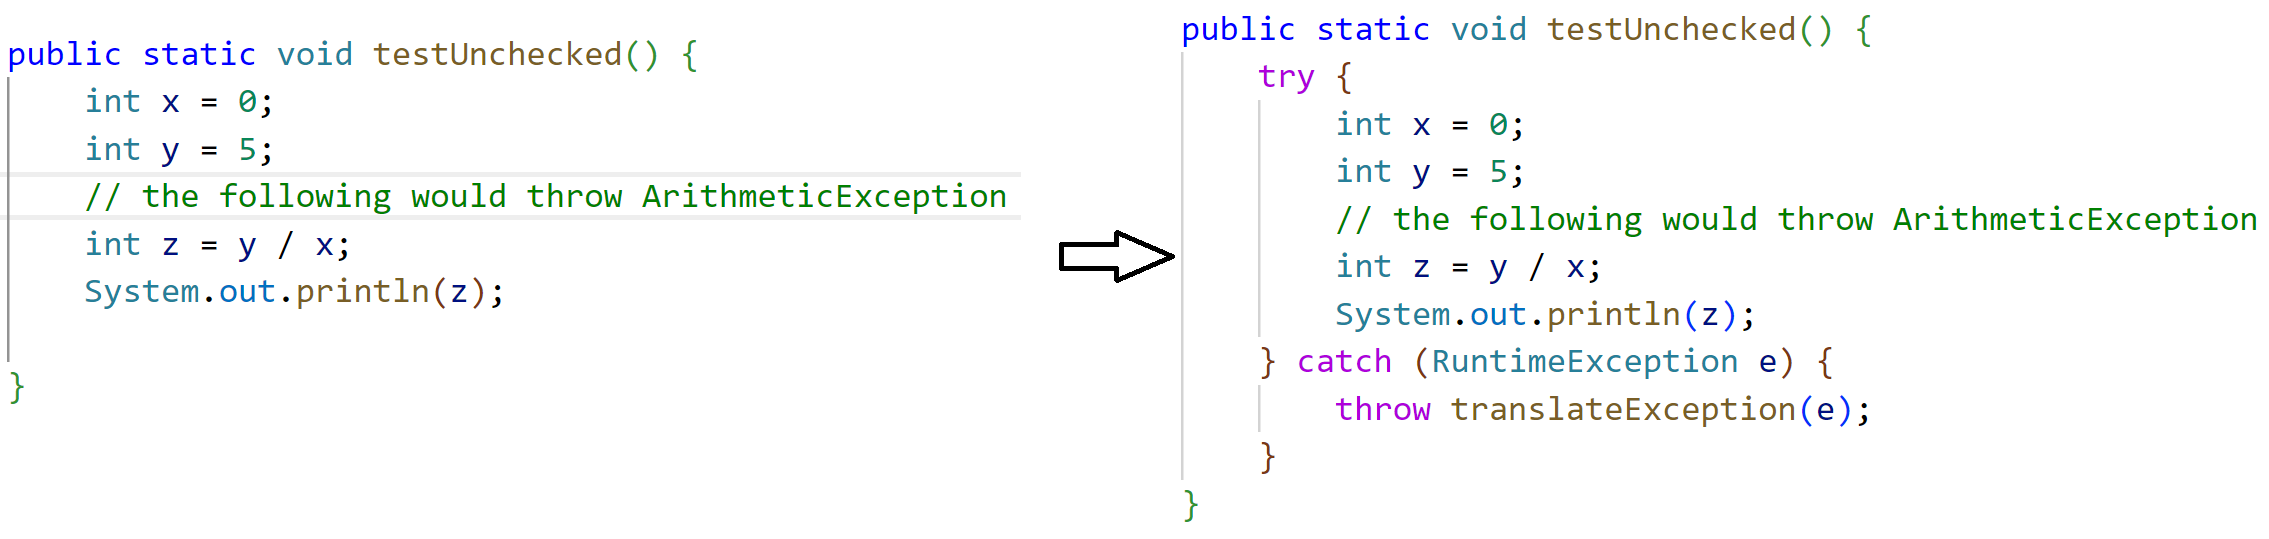
\includegraphics[width=15cm]{ch3-images/unchecked.png}
\caption{An example of a generated code for Unchecked Exceptions}
\label{fig:An example of a generated code for Unchecked Exceptions}
\end{figure} 

To handle Checked Exceptions, I override the visitMethodDeclaration and visitConstructorDeclaration to determine the types of exceptions being thrown and then surround the body of the method or the constructor with try/catch and catch only those exceptions and perform the translation as done with the Unchecked Exceptions. For example:

\begin{figure}[H]
\centering
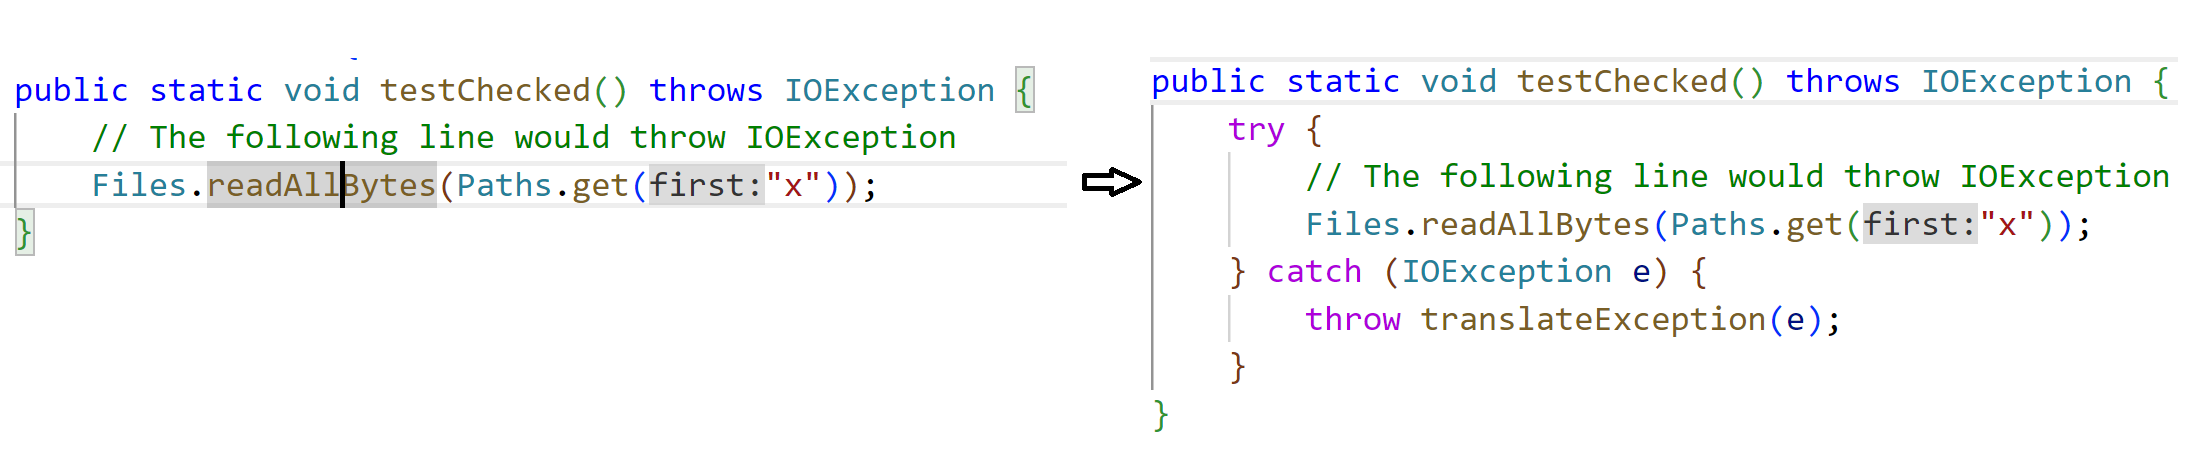
\includegraphics[width=15cm]{ch3-images/checked.png}
\caption{An example of a generated code for Checked Exceptions that is not Caught}
\label{fig:An example of a generated code for Checked Exceptions that is not Caught}
\end{figure} 

Moreover, I override visitCatchClause and visitVariableDeclaratorId to create a new exception variable in the catch block which has the exception translated by the Exception Helper. This is done when the block is already surrounded by a try/catch statement. For Example:

\begin{figure}[H]
\centering
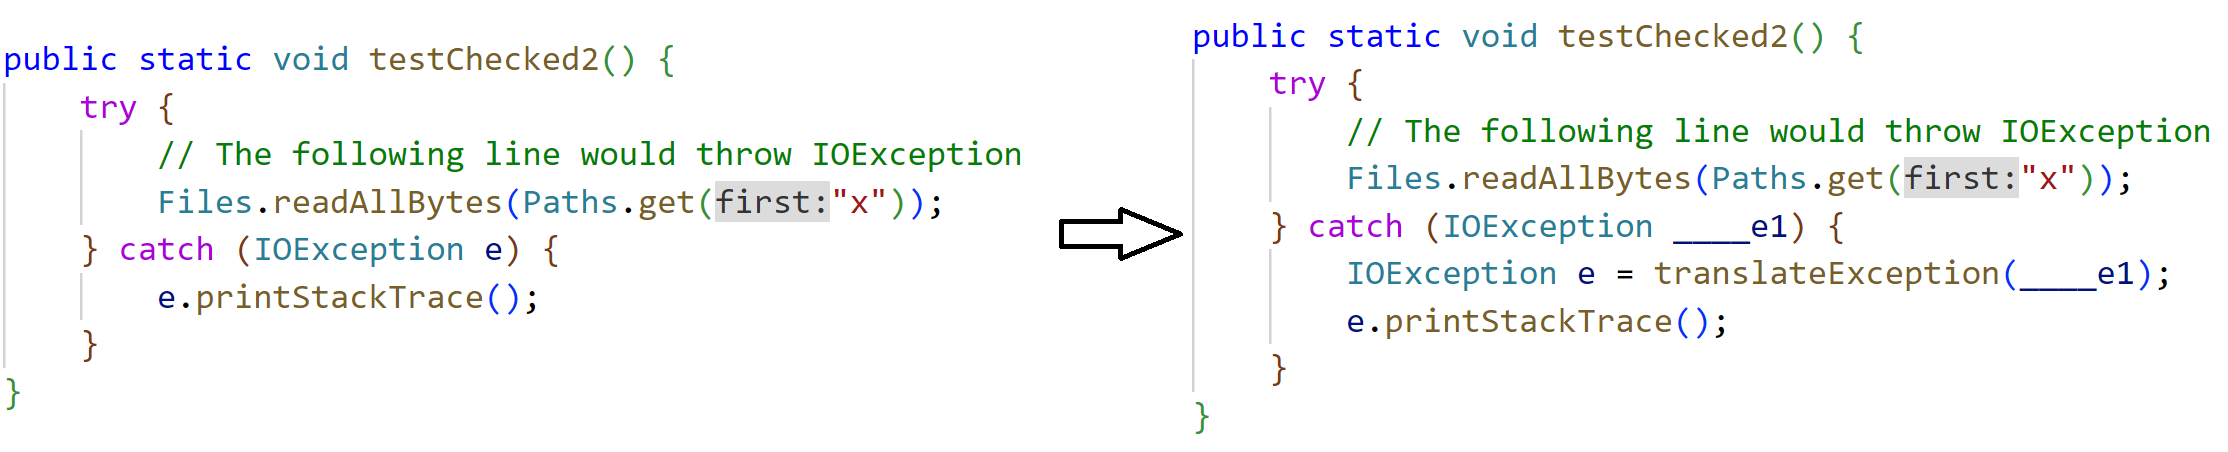
\includegraphics[width=15cm]{ch3-images/checked2.png}
\caption{An example of a generated code for Checked Exceptions that is already Caught}
\label{fig:An example of a generated code for Checked Exceptions that is already Caught}
\end{figure} 

If there is an uncaught exception in the program, Java would call printStackTrace method and then terminates the program. The printStackTrace provided by the Java runtime would print the stack trace and exception class name in English, so I use the visitMethodDeclaration to surround the main method with a try/catch that calls my own implementation of printStackTrace in the Exception Helper component.
\subsubsection{Transpiler}
The Transpiler is used to read the source code file, then calls the lexer to produce the tokens, then calls the parser to generate the parse tree, then finally the java generator traverses the tree to generate the code. It can optionally generate a source map file that maps the line numbers in the source files to those in the target file. It can also optionally generate a JSON file containing all the translated identifiers. This file is embedded after compilation by the PostProcessorMojo (which will be discussed later) so it can be used in runtime to translate exceptions (as explained earlier in the Exception Helper section).

The Transpiler works based on some transpiler options. These options are source language, target language, source encoding, target encoding, the translations object (loaded from translations.guct file), and whether to generate identifiers dictionary or source maps.

Here is an example of the Bubble Sort algorithm transpiled Java code where the source language is Arabic (see figure \ref{fig:Bubble Sort Algorithm in Arabic}):

\begin{figure}[H]
\centering
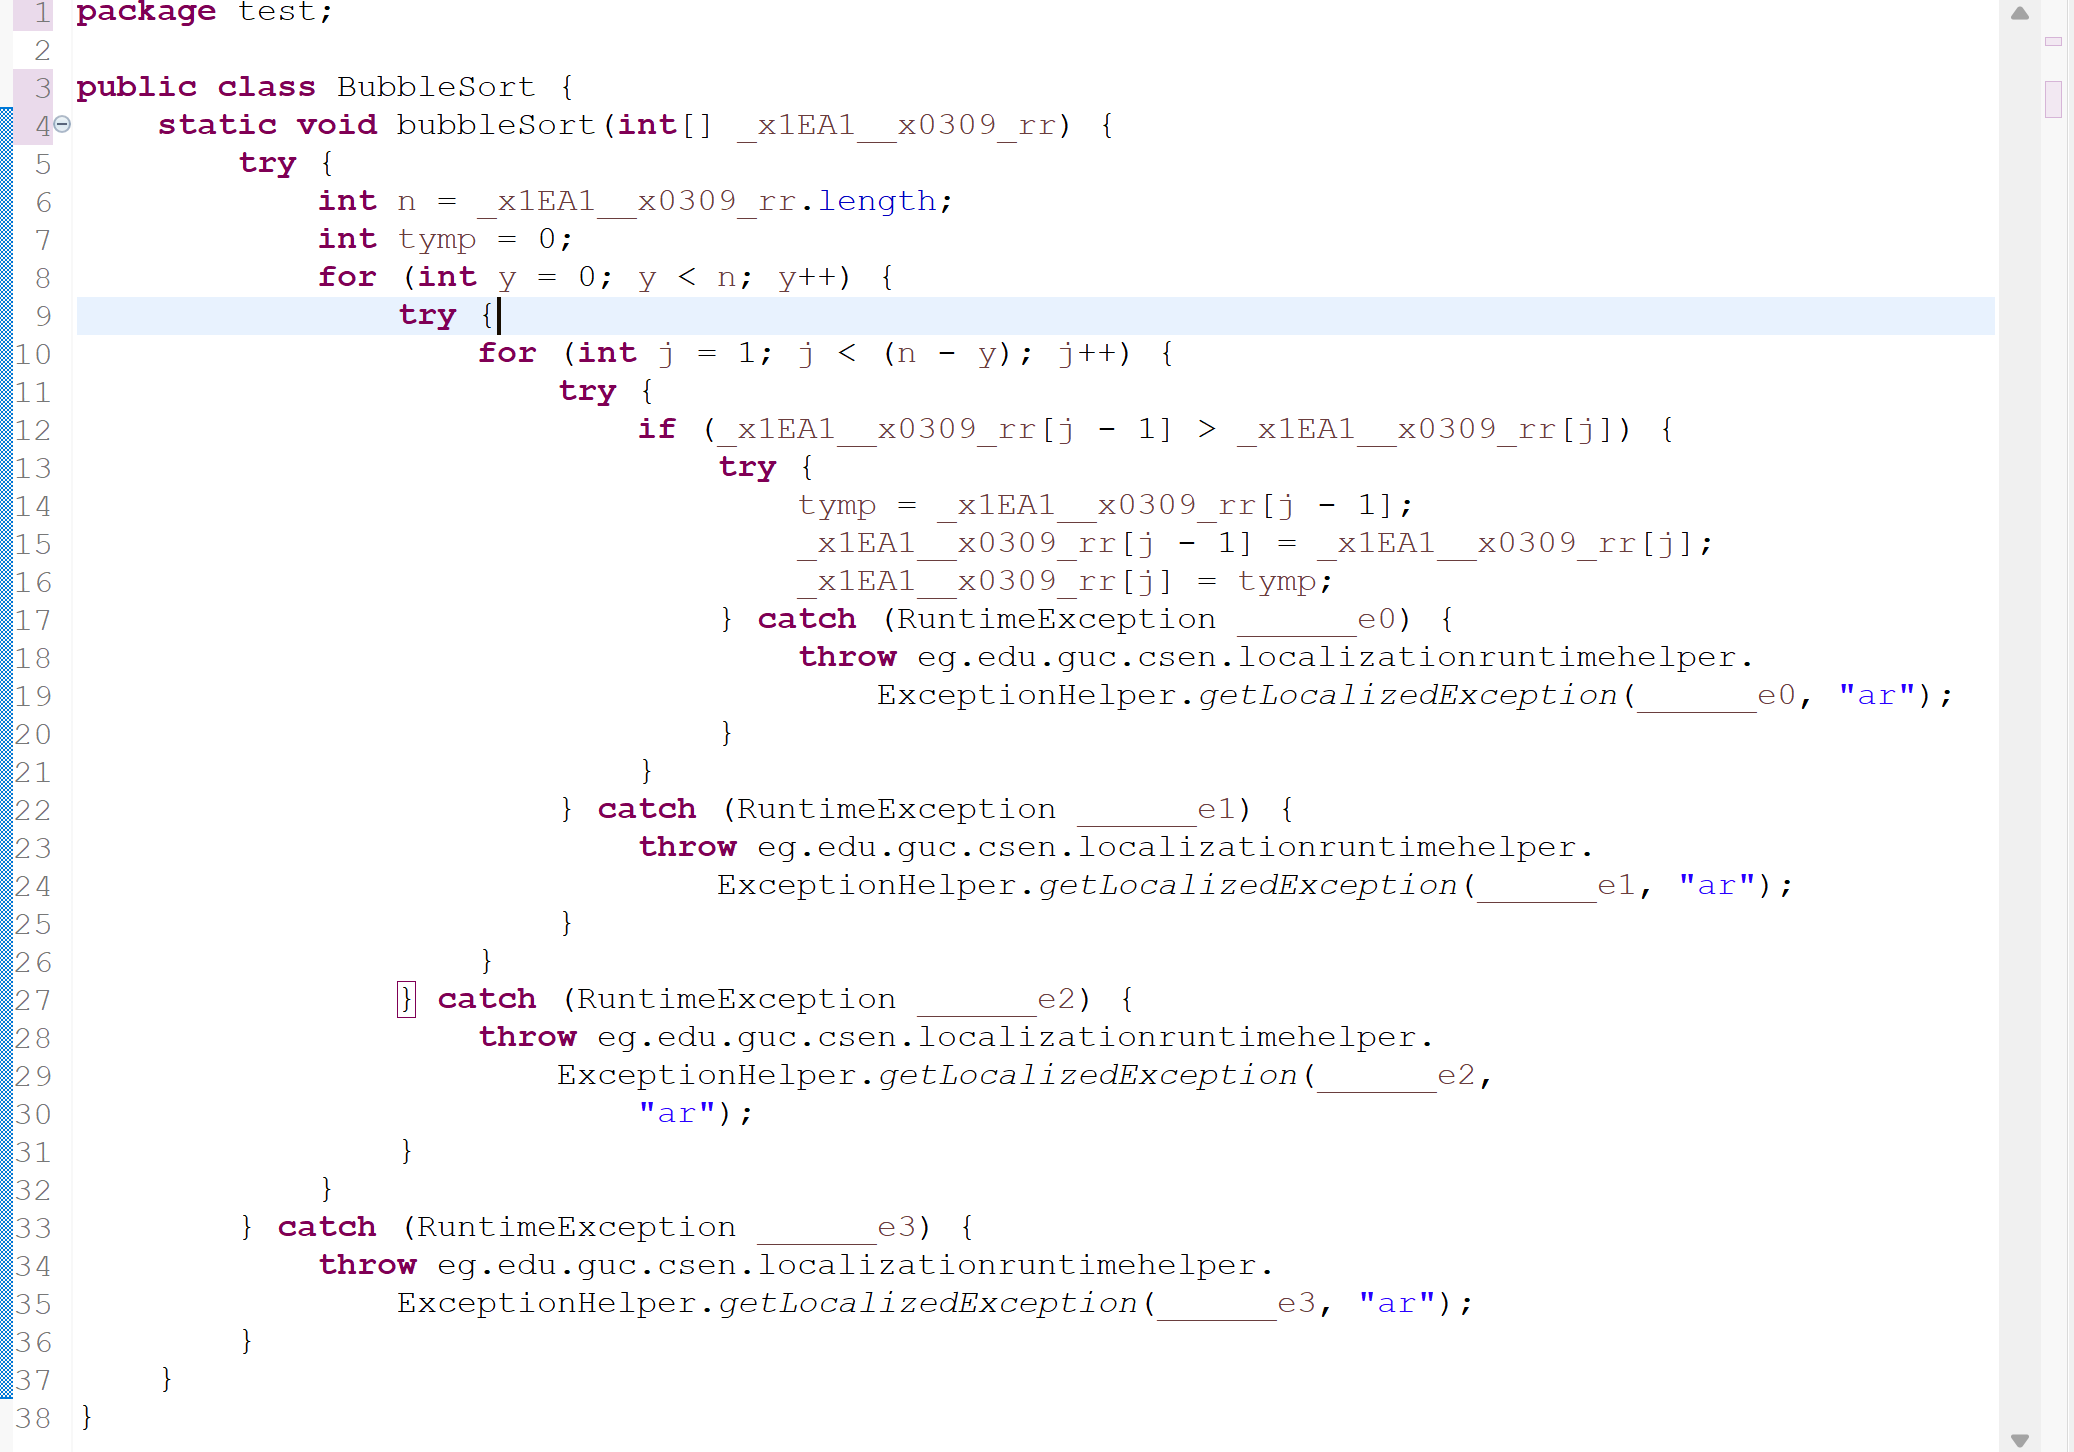
\includegraphics[width=10cm]{ch3-images/bubblesort_transpiled.png}
\caption{The Bubble Sort Algorithm after transpilation}
\label{fig:The Bubble Sort Algorithm after transpilation}
\end{figure} 

\subsection{Maven Plugin Package}
This package is a Maven Plugin that introduces a transpilation step and a post-processing step in the Maven build cycle of the user's project.

\begin{figure}[H]
\centering
\includegraphics[height=8cm]{ch3-images/compilation.png}
\caption{Compilation flowchart}
\label{fig:Compilation flowchart}
\end{figure} 

\subsubsection{Third Party packages}
\begin{enumerate}
    \item \textbf{org.apache.maven.maven-plugin-api}: It contains a base class for Mojos. A Mojo is an executable goal that runs during the maven build cycle.
    \item \textbf{org.apache.maven.plugin-tools.maven-plugin-annotations}: This library provides annotations to mark fields in a Mojo Class as parameters that can be read from the Maven project file (pom.xml).
    \item \textbf{org.apache.maven.maven-project}: This library is used to read Maven project object model files.
    \item \textbf{org.codehaus.plexus.plexus-compiler-api}: This library is used to scan the project's folder for .guc files and process inclusions and exclusions.
    \item \textbf{org.sonatype.plexus.plexus-build-api}: This library provides a build context that checks whether the output files are up to date to avoid unnecessary transpilation steps.
    \item \textbf{org.ow2.asm}: This library provides APIs for reading and writing in Java .class files. This is used by the PostProcessorMojo to write the source map and the identifiers dictionary in the .class file.
\end{enumerate}
\subsubsection{TranspilerMojo}
This Mojo is executed by default in the generate-source phase during the Maven build lifecycle (i.e. before the Java compiler compiles the .java files). It scans all .guc files found in the src folder of the user's project and transpiles each of them to Java using the Transpiler component (discussed earlier). It also generates source maps and identifier dictionaries for each transpiled file which are used by the PostProcessorMojo in a later phase. The Java files (.java), the source map files (.java.smap), and the identifier files (.java.identifiers) are all generated and written in the target/generated-sources/guc folder in the user's project. The PomHelper component (discussed earlier in the Eclipse Plugin section) makes the necessary changes to the project's pom.xml to make sure that the TranspilerMojo is executed and the generated files are included in the Java compilation.
\subsubsection{PostProcessorMojo}
This Mojo is executed by default in the compile phase during the Maven build lifecycle (i.e. after the Java compiler compiles the .java files to .class files). It checks for the presence of source map files (.java.smap) or identifier dictionary files (.java.identifiers) and modifies the .class file to embed the contents of these two files in the .class file. The source map file content is added as a SourceDebugExtension class file attribute so that the stack traces of exceptions would list the .guc files as the source of the errors instead of the .java files. The identifiers dictionary is added as a custom .class file attribute named ``IdentifiersDictionary". This dictionary is used by the Exception Helper component to translate the exceptions' class names and stack traces. 
\section{Deploying and Packaging}
To allow users to access the Maven dependencies and plugins and also the Eclipse Plugin, I deploy them to repositories hosted on the cloud. 
\subsection{Plugin Feature Project}
This is an Eclipse project provided by the Eclipse Plugin SDK. I use this project to package the Eclipse Plugin and its dependencies as a feature that can be downloaded in Eclipse. 
\subsection{Plugin Site Project}
This is an Eclipse project provided by the Eclipse Plugin SDK. I use this project to create the static files containing the downloadable features which will be served by the Eclipse Repository Website. 
\subsubsection{Hosting the Repositories}
To host my repositories, I did the following steps:

 \begin{figure}[H]
    \centering
    \includegraphics{ch3-images/deployment.png}
    \caption{Repository Hosting}
    \label{fig: Repository Hosting}
 \end{figure}

\begin{enumerate}
    \item I registered the domain ``languageslocalization.com" with the registrar ``GoDaddy".
    \item I created a virtual machine to host the sites ``maven.languageslocalization.com", and ``eclipse.languageslocalization.com". I used Linode as the cloud hosting provider. 
    \item I used Reposilite which is an open-source lightweight repository manager for Maven artifacts written in Java to host the Maven repository maven.languageslocalization.com. Moreover, I used nginx as a reverse proxy to Reposilite to provide \ac{SSL}/\ac{TLS} functionality.
    \item I used nginx to serve the static files generated by the plugin site project using the URL eclipse.languageslocalization.com.
    \item I used Certbot to configure, install, and renew the SSL/TLS certificate.
\end{enumerate}
\subsection{Plugin Installation}
To test the plugin, I created a \ac{VM} and installed Eclipse IDE to test all functionalities and features of the Eclipse Plugin. To install the plugin, a couple of steps must be done:

\begin{enumerate}
    \item After opening Eclipse, I must go to the help item in the menu bar and select ``Install New Software" as shown in the following figure:

    \begin{figure}[H]
        \centering
        \includegraphics{ch3-images/installsoftware.png}
        \caption{Installing new software}
        \label{fig: Installing New Software}
    \end{figure}

    \item After selecting ``Install New Software", I must enter the \ac{URL} ``https://www.languageslocalization.com" to add my plugin repository as shown in the following figure:

    \begin{figure}[H]
        \centering
        \includegraphics{ch3-images/addplugin.png}
        \caption{Adding plugin repository}
        \label{fig: Adding plugin repository}
    \end{figure}

    \item Finally, I must select my plugin and select ``Finish" to complete the installation and Eclipse will be restarted with my plugin added.
    
\end{enumerate}
\chapter{Conclusion}\label{chap:concl}

Conclusion

\appendix
\renewcommand{\appendixtocname}{Appendix}
\renewcommand{\appendixpagename}{\appendixtocname}
\addappheadtotoc
\setboolean{@twoside}{false}
\appendixpage

\chapter{Lists}
\addcontentsline{toc}{section}{List of Abbreviations}
\begin{acronym}[\hspace{3cm}]
  \acro{ac}[AC]{Acronym Without Citation}
  \acro{ac2}[AC2]{Acronym With Citation \cite{citeKey2}}
\end{acronym}
\clearpage
\listoffigures
\addcontentsline{toc}{section}{List of Figures}
% \listoftables
% \addcontentsline{toc}{section}{List of Tables}


\bibliographystyle{plain}
\bibliography{bachelor}
\addcontentsline{toc}{chapter}{References}

\end{document}
